\documentclass[a4paper,12pt]{article}
\usepackage{graphicx}
\usepackage[spanish]{babel}
\usepackage{geometry}
\usepackage[utf8]{inputenc}
\usepackage{listings}
\usepackage{xcolor} % colores en codigo
\usepackage{wrapfig}   % Para permitir que el texto envuelva la imagen
%\usepackage[center]{background}
\geometry{left=2.54cm, right=2.54cm, top=2.54cm, bottom=2.54cm}
\renewcommand{\lstlistingname}{Código}
\lstdefinelanguage{JavaScript}{
  keywords={break, case, catch, continue, debugger, default, delete, do, else, finally, for, function, if, in, instanceof, new, return, switch, this, throw, try, typeof, var, void, while, with, let, const},
  keywordstyle=\color{blue}\bfseries,
  ndkeywords={class, export, boolean, throw, implements, import, this},
  ndkeywordstyle=\color{magenta}\bfseries,
  identifierstyle=\color{black},
  sensitive=true,
  comment=[l]{//},
  morecomment=[s]{/*}{*/},
  commentstyle=\color{gray}\ttfamily,
  stringstyle=\color{green!50!black},
  morestring=[b]',
  morestring=[b]",
  inputencoding=utf8,
  extendedchars=true,
  literate={á}{{\'a}}1 {é}{{\'e}}1 {í}{{\'i}}1 {ó}{{\'o}}1 {ú}{{\'u}}1
           {Á}{{\'A}}1 {É}{{\'E}}1 {Í}{{\'I}}1 {Ó}{{\'O}}1 {Ú}{{\'U}}1
           {ñ}{{\~n}}1 {Ñ}{{\~N}}1 {ü}{{\"u}}1 {Ü}{{\"U}}1
}

\lstdefinelanguage{SQL}{
  keywords={SELECT, FROM, WHERE, INSERT, UPDATE, DELETE, CREATE, TABLE, PRIMARY, KEY, FOREIGN, REFERENCES, NOT, NULL, AUTO_INCREMENT, DEFAULT, CONSTRAINT, CHECK, ENGINE, CHARSET, COLLATE, CASCADE, int, float, date, time, tinyint},
  keywordstyle=\color{blue}\bfseries,
  identifierstyle=\color{black},
  sensitive=false,
  comment=[l]{--},
  morecomment=[s]{/*}{*/},
  commentstyle=\color{gray}\ttfamily,
  stringstyle=\color{green!50!black},
  morestring=[b]',
  morestring=[b]",
  inputencoding=utf8,
  extendedchars=true,
  literate={á}{{\'a}}1 {é}{{\'e}}1 {í}{{\'i}}1 {ó}{{\'o}}1 {ú}{{\'u}}1
           {Á}{{\'A}}1 {É}{{\'E}}1 {Í}{{\'I}}1 {Ó}{{\'O}}1 {Ú}{{\'U}}1
           {ñ}{{\~n}}1 {Ñ}{{\~N}}1 {ü}{{\"u}}1 {Ü}{{\"U}}1
}

\lstdefinelanguage{JSX}{
  keywords={break, case, catch, continue, debugger, default, delete, do, else, finally, for, function, if, in, instanceof, new, return, switch, this, throw, try, typeof, var, void, while, with, let, const, useState, useEffect, React},
  keywordstyle=\color{blue}\bfseries,
  ndkeywords={class, export, boolean, throw, implements, import, this, useState, useEffect, const, let, var},
  ndkeywordstyle=\color{magenta}\bfseries,
  identifierstyle=\color{black},
  sensitive=true,
  comment=[l]{//},
  morecomment=[s]{/*}{*/},
  commentstyle=\color{gray}\ttfamily,
  stringstyle=\color{green!50!black},
  morestring=[b]',
  morestring=[b]",
  morekeywords=[2]{useState, useEffect, setFiltros, setCategorias, setSubcategorias, setProductosFiltrados},
  keywordstyle=[2]\color{purple}\bfseries,
  inputencoding=utf8,
  extendedchars=true,
  literate={á}{{\'a}}1 {é}{{\'e}}1 {í}{{\'i}}1 {ó}{{\'o}}1 {ú}{{\'u}}1
           {Á}{{\'A}}1 {É}{{\'E}}1 {Í}{{\'I}}1 {Ó}{{\'O}}1 {Ú}{{\'U}}1
           {ñ}{{\~n}}1 {Ñ}{{\~N}}1 {ü}{{\"u}}1 {Ü}{{\"U}}1
}

\lstset{
  inputencoding=utf8,
  extendedchars=true,
  language=JavaScript,
  backgroundcolor=\color{gray!10},
  basicstyle=\ttfamily\footnotesize,
  numbers=left,
  numberstyle=\tiny\color{gray},
  stepnumber=1,
  numbersep=5pt,
  showstringspaces=false,
  breaklines=true,
  frame=single,
  tabsize=2,
  literate={á}{{\'a}}1 {é}{{\'e}}1 {í}{{\'i}}1 {ó}{{\'o}}1 {ú}{{\'u}}1
           {Á}{{\'A}}1 {É}{{\'E}}1 {Í}{{\'I}}1 {Ó}{{\'O}}1 {Ú}{{\'U}}1
           {ñ}{{\~n}}1 {Ñ}{{\~N}}1 {ü}{{\"u}}1 {Ü}{{\"U}}1,
}
\usepackage{setspace}
\usepackage{caption}   % Para subtítulos
\usepackage{float}  % Agregar en el preámbulo
\usepackage[colorlinks=true,linkcolor=black,urlcolor=blue,citecolor=black]{hyperref}  % Para habilitar enlaces
\usepackage{cite} % citas numericas compactas

\begin{document}
\singlespacing
\thispagestyle{empty}

% --- Logo UAM en esquina superior izquierda ---
\noindent

\includegraphics[width=3cm]{./Logos/uamlog.png}

\vspace{-1cm} % Espacio entre el logo y el texto institucional

% --- Encabezado institucional ---
\begin{center}
\renewcommand{\baselinestretch}{2}\selectfont
\textbf{\Large UNIVERSIDAD AUTÓNOMA METROPOLITANA}\\[0.3cm]
\renewcommand{\baselinestretch}{1}\selectfont

    \textbf{\LARGE Unidad Cuajimalpa}\\[0.3cm]
    \textbf{\Large División de Ciencias Naturales e Ingeniería}\\[0.3cm]
    \textbf{\Large Licenciatura en Ingeniería en Computación}\\[2cm]
\end{center}
 
% --- Título del proyecto ---
\begin{center}
    \renewcommand{\baselinestretch}{2}\selectfont
        \textbf{\huge Punto de Venta Vinculado con un Bot de Discord}\\[0.7cm]
        \renewcommand{\baselinestretch}{1}\selectfont
    \textbf{\Large Proyecto Terminal}\\[3cm]
\end{center}

% --- Autor ---
\begin{flushleft}
    \textbf{\Large Autor:}\\[0.3cm]
    \textbf{\Large Álvaro Arturo Ramírez Arriaga}\\[2cm]
\end{flushleft}

% --- Asesores ---
\begin{flushleft}
    \textbf{\Large Asesores:}\\[0.3cm]
    \textbf{\Large Dr. José Netz Romero Durán}\\[0.2cm]
    \textbf{\Large Mtra. Núñez Reyes Alba Rocío}\\[2cm]
\end{flushleft}

% --- Fecha ---
\vfill
\begin{center}
    \textbf{\Large Ciudad de México, Agosto 2025}
\end{center}

\newpage

\tableofcontents
\newpage
\renewcommand\thesection{\arabic{section}}%reconfiguracion a arabico de las secciones

\section{Introducción}

En la actualidad, la digitalización de los procesos comerciales ha transformado la manera en que las empresas y los consumidores interactúan. Las plataformas de mensajería instantánea y redes sociales, como Discord, han dejado de ser simples herramientas de comunicación para convertirse en espacios donde se pueden gestionar comunidades, ofrecer soporte y hasta realizar transacciones comerciales. Este proyecto surge de la necesidad de aprovechar estas plataformas modernas para mejorar la experiencia de compra y la gestión de ventas en pequeños negocios y emprendimientos.\\

El objetivo principal de este trabajo es el desarrollo de un sistema de punto de venta (POS) en línea que se integra de manera nativa con un bot de Discord. Esta integración permite centralizar la comunicación entre clientes y vendedores, automatizar notificaciones sobre compras y suscripciones, y facilitar la gestión de pedidos en tiempo real. El sistema está diseñado para que los usuarios puedan autenticarse utilizando su cuenta de Discord, navegar por un catálogo de productos, agregar artículos a su carrito, realizar pagos seguros mediante PayPal y recibir notificaciones automáticas sobre sus compras directamente en Discord.\\

El desarrollo del proyecto abarca varias áreas tecnológicas: el frontend está construido con React, proporcionando una interfaz moderna, responsiva y fácil de usar; el backend utiliza Node.js y Express para gestionar la lógica de negocio y la comunicación con la base de datos MySQL, donde se almacena toda la información relevante de usuarios, productos, carritos y tickets de compra. La integración con Discord se realiza mediante la librería Discord.js, que permite crear un bot capaz de interactuar con los usuarios, responder a comandos y enviar notificaciones personalizadas. Además, se implementa la autenticación OAuth2 de Discord para garantizar la seguridad y simplicidad en el acceso de los usuarios.\\

Uno de los aspectos más importantes del sistema es la automatización de notificaciones: cada vez que un usuario realiza una compra, se genera un ticket en la base de datos con una bandera especial que indica que está pendiente de notificación. El bot de Discord revisa periódicamente estos tickets y, al encontrar nuevos, envía mensajes directos a los usuarios con los detalles de su compra, asegurando que la información llegue de manera rápida y directa, incluso si el usuario no revisa su correo electrónico.\\

El proyecto también aborda retos importantes, como la gestión segura de sesiones mediante cookies, la protección de datos sensibles, la integración de pagos electrónicos y el manejo de las limitaciones impuestas por la API de Discord en cuanto al envío de mensajes. 

\newpage

\subsection{Planteamiento del Problema}

En la actualidad se ha visto un crecimiento en la preferencia de las personas por las redes sociales y plataformas de mensajería instantánea como Discord\footnote{Discord es una plataforma de comunicación diseñada para comunidades que permite mensajería de texto, voz y video. Disponible en: \url{https://discord.com}}, que combina comunidad, mensajería y redes sociales. Actualmente, muchas tiendas envían actualizaciones importantes únicamente por correo, lo que resulta en que los mensajes se ignoren o queden en carpetas de spam.\\

El correo electrónico genera fragmentación de la información y su efectividad ha disminuido considerablemente. Según Campaign Monitor, la tasa de apertura de correos comerciales es de apenas 21.33\%~\cite{campaignmonitor}, mientras que las notificaciones por aplicaciones de mensajería como WhatsApp alcanzan tasas de apertura del 90\%~\cite{mma2023}. Por esta razón, muchas empresas han comenzado a enviar notificaciones de compras y actualizaciones por redes sociales como WhatsApp, especialmente dirigidas a usuarios más jóvenes que prefieren estas plataformas.\\

Recientemente, las redes sociales han empezado a emplear mensajes automatizados o bots para agilizar las interacciones con los usuarios, evitando así que estos esperen a que una persona responda. Estos bots son software diseñado para realizar tareas específicas de forma repetida a una mayor velocidad que un ser humano; esto permite agilizar muchas tareas simples como enviar informes y/o mensajes.\\

Este proyecto planteó integrar un bot de Discord con una tienda en línea para centralizar la comunicación entre cliente y vendedor en la red social mencionada. Y así, abordar dos problemas clave: la dispersión de la comunicación y la falta de visibilidad de la información de compra.\\ 
 
El bot que se planteó para este proyecto pretende realizar notificaciones en tiempo real sobre pagos, actualizaciones de pedidos y recordatorios de suscripciones, facilitando la visibilidad de la compra.

\newpage

\section{Objetivos}
En este apartado se presentan los objetivos planteados para guiar el desarrollo del proyecto y proponer una solución tecnológica para la gestión de compras y suscripciones mediante un bot de Discord.
\subsection{Objetivo General}
Desarrollar un sistema que permita el almacenamiento y consulta de los datos de compra de un punto de venta a través de un bot de Discord. \\

\subsection{Objetivos Específicos}
Para este proyecto se tienen los siguientes objetivos específicos. \\

1.- Configurar una base de datos que almacene y gestione la información de compras y suscripciones.\\

2.- Integrar un bot de Discord que permita realizar consultas a la base de datos.\\

3.- Desarrollar un sistema de notificaciones automatizadas.\\

4.- Evaluar las funcionalidades del sistema.\\

5.- Implementar un punto de venta.\\

\newpage

\section{Estado del Arte}
Analizaremos sitios que cuenten con características o funcionalidades similares a las que usaremos para el proyecto que se va a desarrollar: las herramientas a analizar serán PayPal (forma de pago), bot de Discord MEE6, proyecto Tienda Virtual, Uniformes Escolares y Facebook Market.\\

\subsection{PayPal}

El método de pago de PayPal se basa principalmente en una implementación a través de su API, más que en el diseño de una interfaz propia. Esta API requiere información como la solicitud de pago, el precio del producto y la cuenta de PayPal a la que se debe depositar el dinero una vez que se complete la transacción. Por lo tanto, la única tarea que debe implementar el programador es la integración de la API y el botón para invocar el proceso de pago de PayPal.\\

\begin{figure}[H]
  \centering
  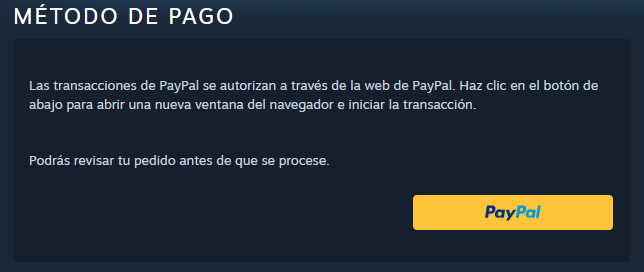
\includegraphics[width=0.7\textwidth]{./Imagenes/pago1.png}
  \caption{Botón de método de pago PayPal.\cite{paypal}}
  \label{fig:pago1}
\end{figure}

El botón de la figura~\ref{fig:pago1} no es más que una conexión de la página web, la sección de pago con el verdadero gestor de la transacción, como es PayPal, mediante la API.

\newpage
Una vez llamada la API de PayPal, esta nos llevará a una ventana emergente (figura~\ref{fig:pago2}) donde se nos pedirá ingresar los datos de la cuenta de la plataforma PayPal para poder continuar con el cobro del servicio. Esta interfaz ya no es necesario crearla.\\

\begin{figure}[H]
  \centering
  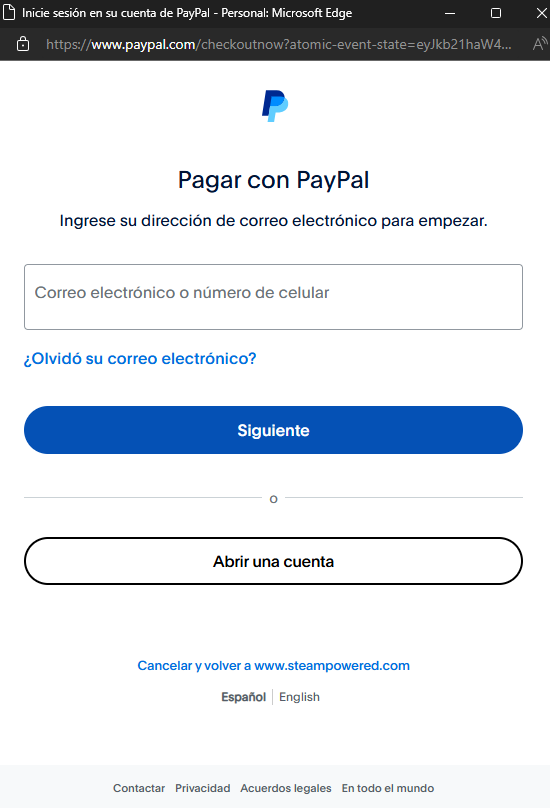
\includegraphics[width=0.5\textwidth]{./Imagenes/pago2.png}
  \caption{Formulario de inicio de sesión de PayPal.\cite{paypal}}
  \label{fig:pago2}
\end{figure}

La figura~\ref{fig:pago2} muestra la interfaz para la autenticación desde la API de PayPal, donde el usuario debe autenticarse con su cuenta de PayPal para acceder al sistema. Se utiliza el sistema OAuth2 de PayPal para este propósito.

El pago entraría casi de inmediato, solo faltaría confirmar el pago para que se realice el cobro del servicio y finalizaría así el cobro por vía PayPal.

\newpage
\subsection{MEE6 Bot Discord}

El bot MEE6 cuenta con muchas características interesantes para nosotros, pero en este proyecto nos centraremos en la posibilidad de enviar notificaciones de recordatorios por un canal específico o por mensaje directo al usuario.

\begin{figure}[H]
  \centering
  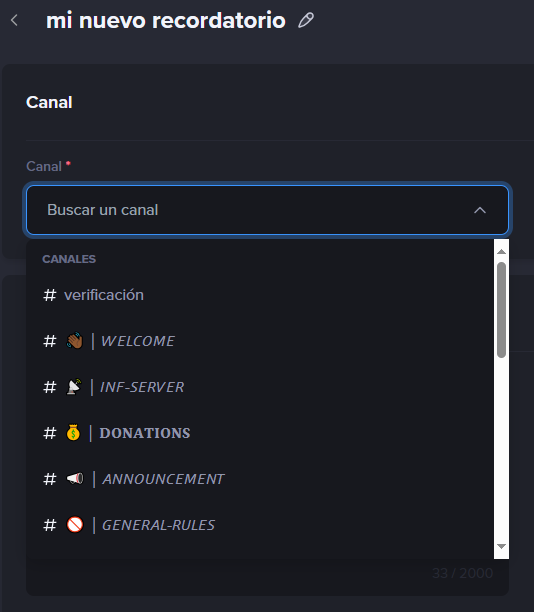
\includegraphics[width=0.6\textwidth]{./Imagenes/recordatorio1.png}
  \caption{Selección de canal para recordatorio.\cite{mee6}}
  \label{fig:recordatorio1}
\end{figure}

En la ventana de la figura~\ref{fig:recordatorio1} podremos seleccionar en qué canal queremos que se genere el recordatorio que vamos a colocar. Esto es útil para aplicar recordatorios para un grupo de personas con roles específicos dentro del servidor de Discord. De esta forma, solo llegarán los recordatorios a las personas que queremos que reciban estos mensajes. También podemos poner un auto rol para que ellos decidan si quieren recibir los recordatorios o no, algo similar a cuando te pregunta una empresa si quieres recibir correos de promociones.

\begin{figure}[H]
  \centering
  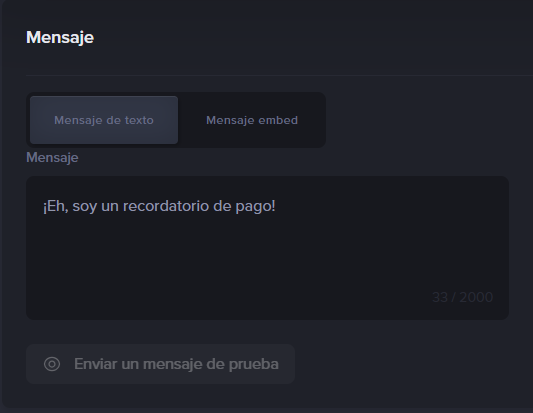
\includegraphics[width=0.6\textwidth]{./Imagenes/recordatorio3.png}
  \caption{Ingreso del mensaje de recordatorio.\cite{mee6}}
  \label{fig:recordatorio2}
\end{figure}

La interfaz de la figura~\ref{fig:recordatorio2} permite ingresar el mensaje que deseamos que los usuarios reciban como recordatorio. En este caso, el mensaje consistirá únicamente en texto, aunque también es posible agregar una imagen para que el bot la publique automáticamente junto con el texto. De esta forma, se puede generar una publicidad mucho más eficaz para los artículos y el público objetivo al que va dirigida.\\

Además, al tener la posibilidad de enviar mensajes directos a los usuarios, podremos notificarles sobre próximas fechas de pago para alguna suscripción activa, o incluso ofrecerles descuentos personalizados.

\newpage
\begin{figure}[H]
  \centering
  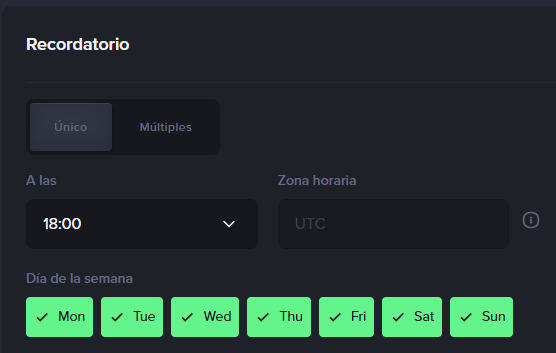
\includegraphics[width=0.7\textwidth]{./Imagenes/recordatorio2.png}
  \caption{Configuración de recordatorios automáticos.\cite{mee6}}
  \label{fig:recordatorio3}
\end{figure}

La función de recordatorio se puede configurar de forma personalizada, como se muestra en la figura~\ref{fig:recordatorio3}. Para que el recordatorio se genere automáticamente a intervalos de tiempo específicos, es necesario indicar el día y la hora. Esta funcionalidad es útil para evitar tener que crear el recordatorio de forma manual cada vez que se desee generar uno similar. En nuestro caso, tomará esta información de una base de datos, donde verificará si es necesario aplicar el recordatorio. En caso de tratarse de una mensualidad, recordará al usuario con 5 días de anticipación, revisando la fecha del siguiente cobro.
\newpage


\subsection{Tienda de Uniformes Escolares}

En este proyecto desarrollado en la Universidad Abierta de Cataluña se realizó una tienda online de uniformes escolares, del cual tomaremos algunas utilidades de este proyecto como referencia.\\


\begin{figure}[H]
  \centering
  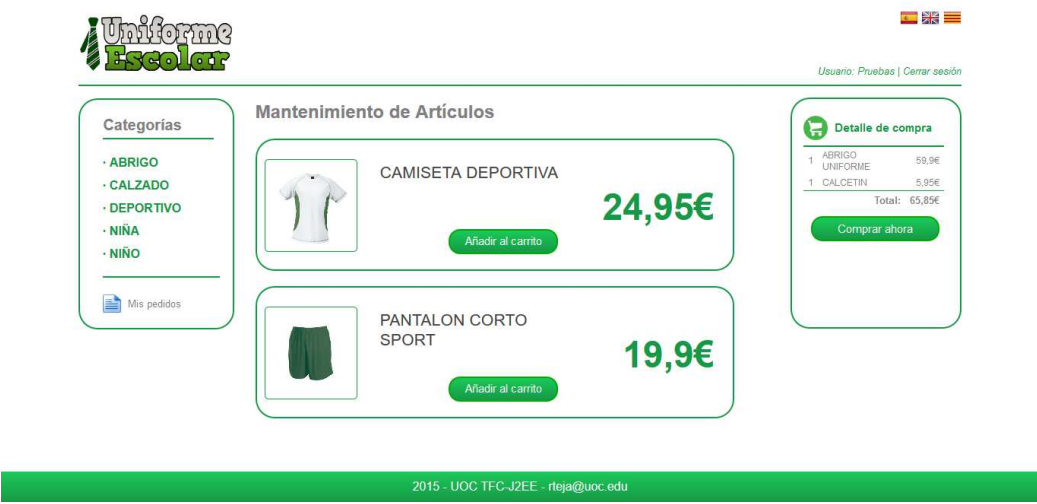
\includegraphics[width=0.8\textwidth]{./Imagenes/UE1.png}
  \caption{Listado de artículos de la tienda de uniformes.\cite{uniformes}}
  \label{fig:ue1}
\end{figure}

 Como podemos ver en la figura~\ref{fig:ue1}, en la interfaz de compra únicamente hace falta dar clic sobre 'añadir al carrito' para poder adquirirlo; también se ve el precio del producto y su nombre.\\

 Del lado izquierdo también se puede apreciar el filtro que se tiene para los productos, de esta forma se tiene una mejor organización sobre lo que está observando el usuario comprador en este momento. Al lado derecho se muestran los productos que han sido añadidos al carrito, así como el precio final de la compra.
 \newpage
 
  En la figura~\ref{fig:ue2} podemos ver qué pasa al darle clic a comprar, ahora nos manda a la página de pago donde saldrán los datos del comprador, en este caso se ve cómo el pago se carga automáticamente a la mensualidad del colegio, en nuestro caso habrá un método de pago para realizar el pago.\\
  
\begin{figure}[H]
  \centering
  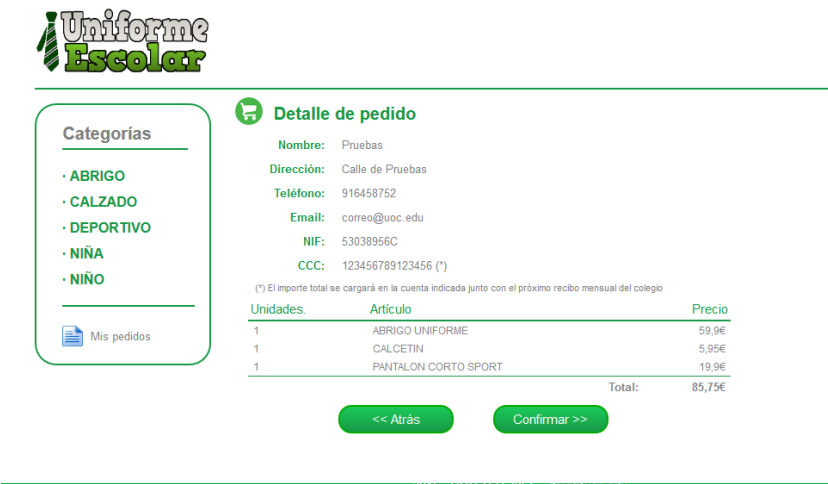
\includegraphics[width=0.8\textwidth]{./Imagenes/UE2.png}
  \caption{Resumen de compra y datos del comprador.\cite{uniformes}}
  \label{fig:ue2}
\end{figure}

Para nuestro proyecto será importante colocar una sección de productos para seleccionarlos y, después de seleccionarlos, colocar una descripción y más imágenes para que el comprador pueda ver y estar más seguro de que se está comprando, al igual que un desglose de su compra total.
\newpage
\clearpage
\subsection{Facebook Marketplace}
Facebook Marketplace también es otra de las plataformas más utilizadas para la compra y venta de productos, por esta razón es una buena referencia para el proyecto.\\

En la figura~\ref{fig:fbm3} podemos ver cómo se muestra la información del vendedor, detalles del producto y algunas especificaciones básicas; no es tan extensa la descripción como en Amazon. Sin embargo, nos da la posibilidad de enviarle un mensaje al comprador para poder preguntarle a él de una forma más directa y personalizada.\\

\begin{figure}[H]
  \centering
  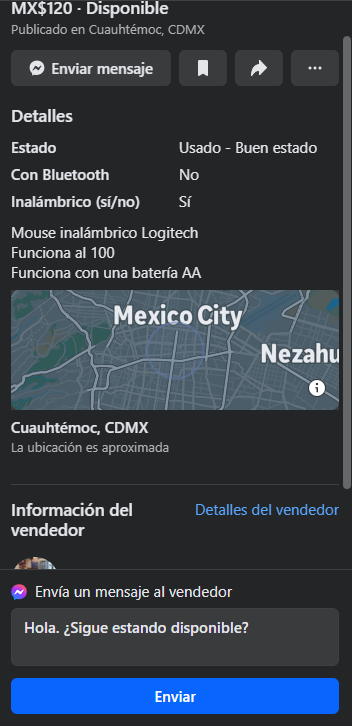
\includegraphics[width=0.35\textwidth]{./Imagenes/FBm3.png}
  \caption{Información del producto y vendedor en Marketplace.\cite{facebook}}
  \label{fig:fbm3}
\end{figure}

La figura~\ref{fig:fbm3} muestra la sección informativa donde se puede ver el detalle del producto, así como la opción de contactar al vendedor.

Si bien esta plataforma está orientada a que terceros vendan sus productos en su tienda, son buenas referencias para este proyecto, al poder tener un trato directo con el vendedor.\\

Este proyecto tomará la idea de poder mandarle mensajes directamente al vendedor, en este caso, el administrador de la tienda, para algunas compras que requieran de más pasos y no solo vender el producto.
\newpage
\subsection{AliExpress}
Algunas tiendas en línea ya utilizan actualmente notificaciones por medio de alguna red social; este es el caso de AliExpress, donde reenvían información básica de tu compra y links para visualizar la información completa de la compra en una página web. Si bien no es el ticket, sí facilita poder verlo sin necesidad de entrar al correo electrónico.\\

La figura~\ref{fig:aliex} ejemplifica una notificación simplificada que recibiría el usuario tras realizar una compra.

\begin{figure}[H]
  \centering
  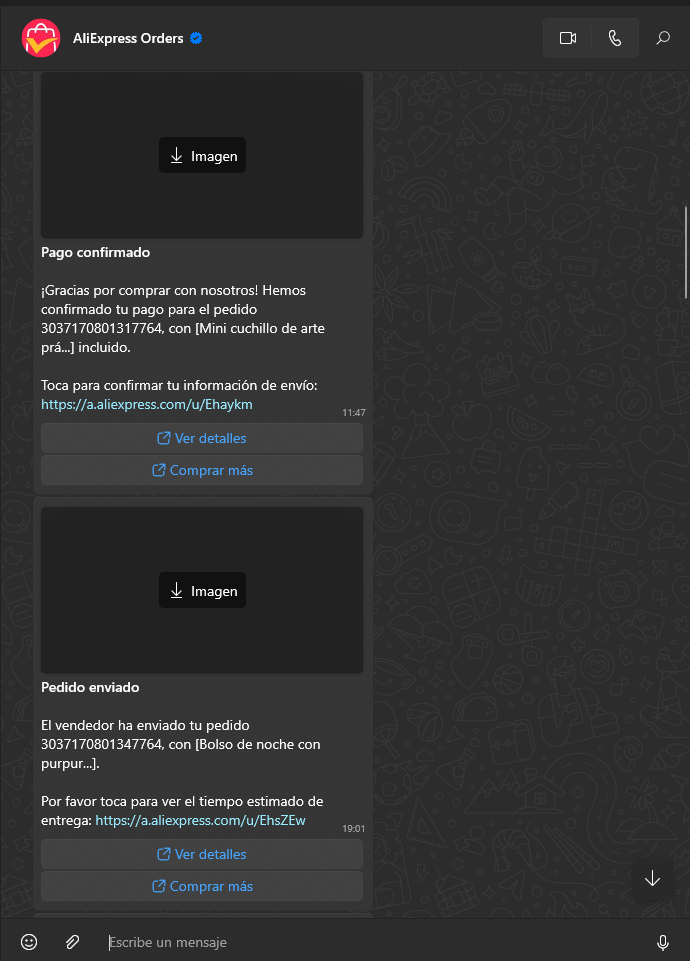
\includegraphics[width=0.5\textwidth]{./Imagenes/aliex.PNG}
  \caption{Notificación de compra reenviada (AliExpress).\cite{aliexpress}}
  \label{fig:aliex}
\end{figure}

Este proyecto busca poder realizar notificaciones mediante una red social como es Discord para centralizar la forma de encontrar la información de compra y contactar con la tienda o persona encargada de esta de una forma mucho más fácil, utilizando únicamente Discord.
\newpage


\section{Definición General del sistema}
En esta sección se describe la arquitectura general del sistema propuesto, así como las tecnologías a utilizar durante el desarrollo del sistema.
\subsection{Propuesta}
Este proyecto propone la creación de un punto de venta en línea integrado con un bot de Discord, con el fin de centralizar la comunicación y optimizar la gestión de compras y suscripciones. La propuesta incluye la implementación de métodos de pago seguros como PayPal, permitiendo a los usuarios realizar transacciones de manera confiable y eficiente.\\

El sistema busca aprovechar la versatilidad y popularidad de Discord como plataforma principal para ofrecer notificaciones en tiempo real sobre pagos, actualizaciones de pedidos y recordatorios de suscripciones. La integración del bot con la tienda en línea permite automatizar completamente las notificaciones de tickets de compra y suscripciones adquiridas, las cuales son enviadas directamente vía Discord a los usuarios correspondientes.\\

El proyecto incluye el diseño y desarrollo de una base de datos robusta para almacenar y consultar información relevante como datos de usuarios, catálogo de productos, historial de compras, tickets generados y estados de notificación. Esta base de datos soporta la integración del bot para realizar consultas y notificaciones automatizadas.\\

También se contempla la implementación de autenticación mediante OAuth2 de Discord, eliminando la necesidad de crear cuentas adicionales y aprovechando la infraestructura existente de la plataforma. El sistema de carritos de compra permite a los usuarios agregar productos, modificar cantidades y proceder al pago de manera intuitiva.\\

Además, se incluye un sistema de notificaciones inteligente que verifica periódicamente nuevos tickets de compra y suscripciones, enviando mensajes personalizados a través del bot de Discord. Esto mejora significativamente la visibilidad de la información de compra y la interacción directa con los usuarios.\\
\newpage
\subsection{Tecnologías}

Las tecnologías para este proyecto serán API PayPal, API Discord, MySQL, Node.js, React. Se explicará cada una de las tecnologías para definir qué funcionalidad van a desempeñar en el proyecto propuesto.
\subsubsection{PayPal}

PayPal es una de las plataformas más populares para pagos en línea, conocida por su facilidad de uso, seguridad y aceptación internacional. Para este proyecto, se ha elegido PayPal debido a su amplia adopción por los usuarios y su capacidad para gestionar pagos transfronterizos de manera eficiente, ofreciendo una ventaja frente a competidores como Mercado Pago.\\

La integración de PayPal en una tienda en línea se realiza principalmente mediante su API. Esta API permite establecer la comunicación entre la tienda y los servidores de PayPal para gestionar las transacciones de manera segura.\\

Una ventaja adicional de PayPal es que proporciona un entorno de pruebas (sandbox) que facilita el desarrollo y testing del sistema. Este entorno permite realizar transacciones simuladas sin manejar dinero real, lo que es ideal para verificar que la integración funciona correctamente y que los mensajes de confirmación de compra se reciben adecuadamente a través de la API. Esto garantiza que el sistema esté completamente funcional antes de implementarlo en producción.\\


\subsubsection{Discord}

Discord es una plataforma de comunicación ampliamente utilizada para la creación y gestión de comunidades temáticas. Originalmente orientada hacia los jugadores, Discord ha evolucionado para ser una herramienta versátil que permite administrar grandes grupos de usuarios gracias a su estructura basada en servidores. En estos servidores, se pueden asignar roles, gestionar permisos y utilizar bots para automatizar diversas tareas, convirtiéndola en una solución ideal para centralizar la interacción entre usuarios y servicios.\\

Discord facilita significativamente el desarrollo de bots mediante su API robusta y bibliotecas especializadas como Discord.js para Node.js. Estas herramientas simplifican la implementación de funcionalidades avanzadas como comandos slash, embeds interactivos, gestión de eventos en tiempo real y notificaciones automáticas.\\

Discord será una herramienta central en este proyecto, gracias a su capacidad para gestionar usuarios y automatizar notificaciones. Se aprovecharán tanto su API como las características de inicio de sesión para integrar la tienda en línea con la plataforma.\\

Se utilizará la OAuth2 API de Discord para implementar un sistema de autenticación seguro y sencillo. Esto permitirá a los usuarios iniciar sesión en la tienda en línea con su cuenta de Discord, sin necesidad de crear un nuevo usuario.

\newpage

\subsubsection{Node.js}

Node.js es un entorno de ejecución que permite ejecutar JavaScript fuera del navegador. Basado en el motor V8 de Google Chrome, Node.js es extremadamente rápido y eficiente, especialmente para aplicaciones que requieren manejo en tiempo real y procesamiento asíncrono.\\

Una de las principales ventajas de Node.js es su capacidad para funcionar como servidor web completo, reemplazando la necesidad de servidores tradicionales como Apache o Nginx en muchos casos. Node.js incluye un servidor HTTP integrado que permite crear aplicaciones web desde cero sin depender de software adicional. Esto facilita significativamente el desarrollo y despliegue de aplicaciones, especialmente en entornos locales donde se puede levantar un servidor completo.\\

Node.js es ideal para aplicaciones que necesitan manejar múltiples solicitudes simultáneamente mediante su arquitectura de eventos no bloqueante. Esta característica lo convierte en la opción perfecta para aplicaciones como bots de Discord que deben responder a eventos en tiempo real, procesar múltiples comandos de usuarios y mantener conexiones persistentes. Su estabilidad permite conservar un buen rendimiento incluso con muchas solicitudes simultáneas.\\

Para este proyecto, Node.js actúa como servidor backend para la tienda en línea, gestionando la lógica de negocio, autenticación y comunicación con la base de datos; y además sirve como plataforma para el bot de Discord mediante la biblioteca Discord.js.\\

\textbf{Discord.js}\\

Discord.js es una biblioteca de Node.js específicamente diseñada para simplificar la interacción con la API de Discord. Esta librería proporciona una abstracción de alto nivel que facilita enormemente el desarrollo de bots, eliminando la complejidad de manejar directamente las conexiones WebSocket y las peticiones HTTP a la API de Discord.\\

Discord.js ofrece características avanzadas como manejo automático de reconexiones, sistema de eventos robusto, tipado para TypeScript, y métodos simplificados para todas las funcionalidades de Discord. Permite implementar fácilmente comandos slash, embeds interactivos con botones y menús desplegables, gestión de roles y permisos, y notificaciones automáticas.\\

En este proyecto, Discord.js permite que el bot pueda registrar comandos dinámicamente, enviar mensajes directos personalizados a los usuarios tras completar una compra y realizar una gestión de eventos en tiempo real como la comprobación de los nuevos tickets creados en la Base de Datos.\\

\subsubsection{React}

React es una biblioteca de JavaScript desarrollada por Facebook, diseñada para construir interfaces de usuario (UI) modernas, interactivas y dinámicas. Se enfoca principalmente en la creación de aplicaciones a través de componentes reutilizables, lo que permite dividir la interfaz en pequeñas piezas independientes y manejables. Esto mejora la organización y el mantenimiento del código; también facilita la reutilización de estos componentes en diferentes partes de la aplicación. En este proyecto, un componente podría encargarse de mostrar los productos de la tienda, otro del carrito de compras y otro de las notificaciones de compra, optimizando así el desarrollo.\\

Una de las características más destacadas de React es el uso del Virtual DOM. Este mecanismo crea una representación en memoria del DOM real, lo que permite que React identifique y actualice solo las partes necesarias de la interfaz en lugar de renderizarla por completo cada vez que hay un cambio. Esto mejora significativamente el rendimiento de la aplicación, especialmente en escenarios donde las actualizaciones en tiempo real son frecuentes, como al agregar productos al carrito o actualizar el estado de un pedido.\\

React fue elegido para este proyecto debido a su escalabilidad y facilidad de mantenimiento. React ofrece un equilibrio ideal entre flexibilidad y robustez, lo que lo convierte en una herramienta esencial para construir una tienda en línea moderna que integre funcionalidades avanzadas como notificaciones en tiempo real y bots automatizados.
\newpage
\subsubsection{MySQL}

MySQL es un sistema de gestión de bases de datos relacional, se utiliza para almacenar, organizar y administrar grandes volúmenes de información en aplicaciones de software. Este sistema utiliza el lenguaje SQL (Structured Query Language) para interactuar con los datos, permitiendo realizar operaciones como consultas, inserciones, actualizaciones y eliminaciones de manera eficiente y estructurada. \\

Una de las principales ventajas de MySQL es su capacidad para manejar grandes cantidades de datos de manera rápida y eficiente. Gracias a su diseño optimizado, MySQL permite realizar consultas complejas que filtran y procesan información específica en cuestión de milisegundos. Esto es crucial en aplicaciones como tiendas en línea, donde se manejan continuamente datos relacionados con usuarios, productos, pedidos y transacciones.\\

Otra característica importante de MySQL es su enfoque en la integridad de los datos y la seguridad. A través de herramientas como Prepared Statements (consultas preparadas), es posible proteger la base de datos contra ataques comunes como la inyección SQL, garantizando que las consultas se ejecuten de forma segura y controlada. Esta funcionalidad es esencial en proyectos que manejan información confidencial, como detalles de usuarios y transacciones económicas.\\

En este proyecto, MySQL se utilizará para gestionar tablas que almacenen información esencial como detalles de los usuarios, productos, pedidos y estados de pago. Además, permitirá realizar operaciones frecuentes, como buscar productos según filtros personalizados, actualizar el estado de un pedido en real tiempo o registrar nuevas transacciones.\\
\newpage
\subsection{Requerimientos Funcionales}
A continuación, se presentan los requerimientos funcionales del proyecto, los cuales describen las acciones y comportamientos que el sistema deberá cumplir para satisfacer las necesidades del usuario y alcanzar los objetivos planteados. Estos requerimientos definen qué funciones específicas realizará el sistema, incluyendo la interacción con el bot de Discord, la gestión de pedidos y la comunicación con los clientes.\\

\subsubsection{Página Web}

- Permitir a los usuarios navegar por los productos disponibles en la tienda virtual.\\

- Permitir a los usuarios autenticarse mediante Discord (OAuth2).\\

- Permitir a los usuarios agregar productos al carrito de compras.\\

- Permitir a los usuarios modificar la cantidad de productos en el carrito y eliminar productos del mismo.\\

- Permitir a los usuarios realizar compras y generar tickets de compra usando PayPal.\\

- Mostrar notificaciones de éxito o error en las operaciones principales (login, agregar al carrito, compra).\\

- Permitir a los usuarios ver su perfil y cerrar sesión.\\

- Mostrar información relevante de los productos (nombre, imagen, precio, categoría).\\

- Permitir la navegación entre diferentes páginas (productos, carrito, perfil).\\

- Integración con un servidor de Discord (botón de invitación y QR).\\

- Permitir que los usuarios puedan realizar pagos electrónicos por PayPal.\\

\subsubsection{Bot Discord}
- Permitir la integración con el servidor de Discord de la tienda virtual.\\

- Responder a comandos básicos de los usuarios /productos.\\

- Notificar en canales específicos cuando se realiza una compra o se genera un ticket en la tienda.\\

- Permitir la gestión de roles o permisos para usuarios que compran productos.\\

- Permitir la consulta de información de productos o tickets desde Discord (si aplica).\\
\newpage
\subsection{Requerimientos no Funcionales}
En esta sección se detallan los requerimientos no funcionales del proyecto, los cuales establecen los criterios de calidad que el sistema debe cumplir.
\subsubsection{Página Web}

- La aplicación debe ser responsiva y funcionar correctamente en dispositivos móviles y de escritorio.\\

- El sistema debe mantener la sesión del usuario mediante cookies seguras.\\

- El backend debe manejar la autenticación de manera segura.\\

- El sistema debe manejar errores y mostrar mensajes claros al usuario.\\

- El sistema debe ser escalable para permitir la integración de nuevas funcionalidades (por ejemplo, más métodos de pago, más categorías).\\

- El sistema debe proteger los datos sensibles y cumplir con buenas prácticas de seguridad.\\

- El backend debe soportar concurrencia y múltiples usuarios simultáneos.\\

- El sistema debe permitir la integración con servicios externos como Discord y PayPal.\\

\subsubsection{Bot Discord}\
- El bot debe estar disponible 24/7 y manejar desconexiones de manera automática.\\

- El código debe estar organizado y documentado para facilitar el mantenimiento.\\

- El bot debe manejar errores y excepciones sin interrumpir su funcionamiento.\\

- El bot debe proteger los tokens y credenciales de acceso.\\

- El bot debe ser escalable para permitir la adición de nuevos comandos o integraciones.\\
\newpage

\section{Diseño del Sistema}
En esta sección se presenta el diseño del sistema, incluyendo diagramas que ilustran la arquitectura, los flujos de interacción y la estructura de la base de datos. Estos diagramas proporcionan una visión clara de cómo se integran los diferentes componentes del sistema y cómo interactúan entre sí para cumplir con los requerimientos funcionales y no funcionales establecidos.
\subsection{Diagrama General}

El diagrama general del sistema muestra los principales componentes y su interacción. A continuación se describen los elementos clave:

\begin{figure}[H]
  \centering
  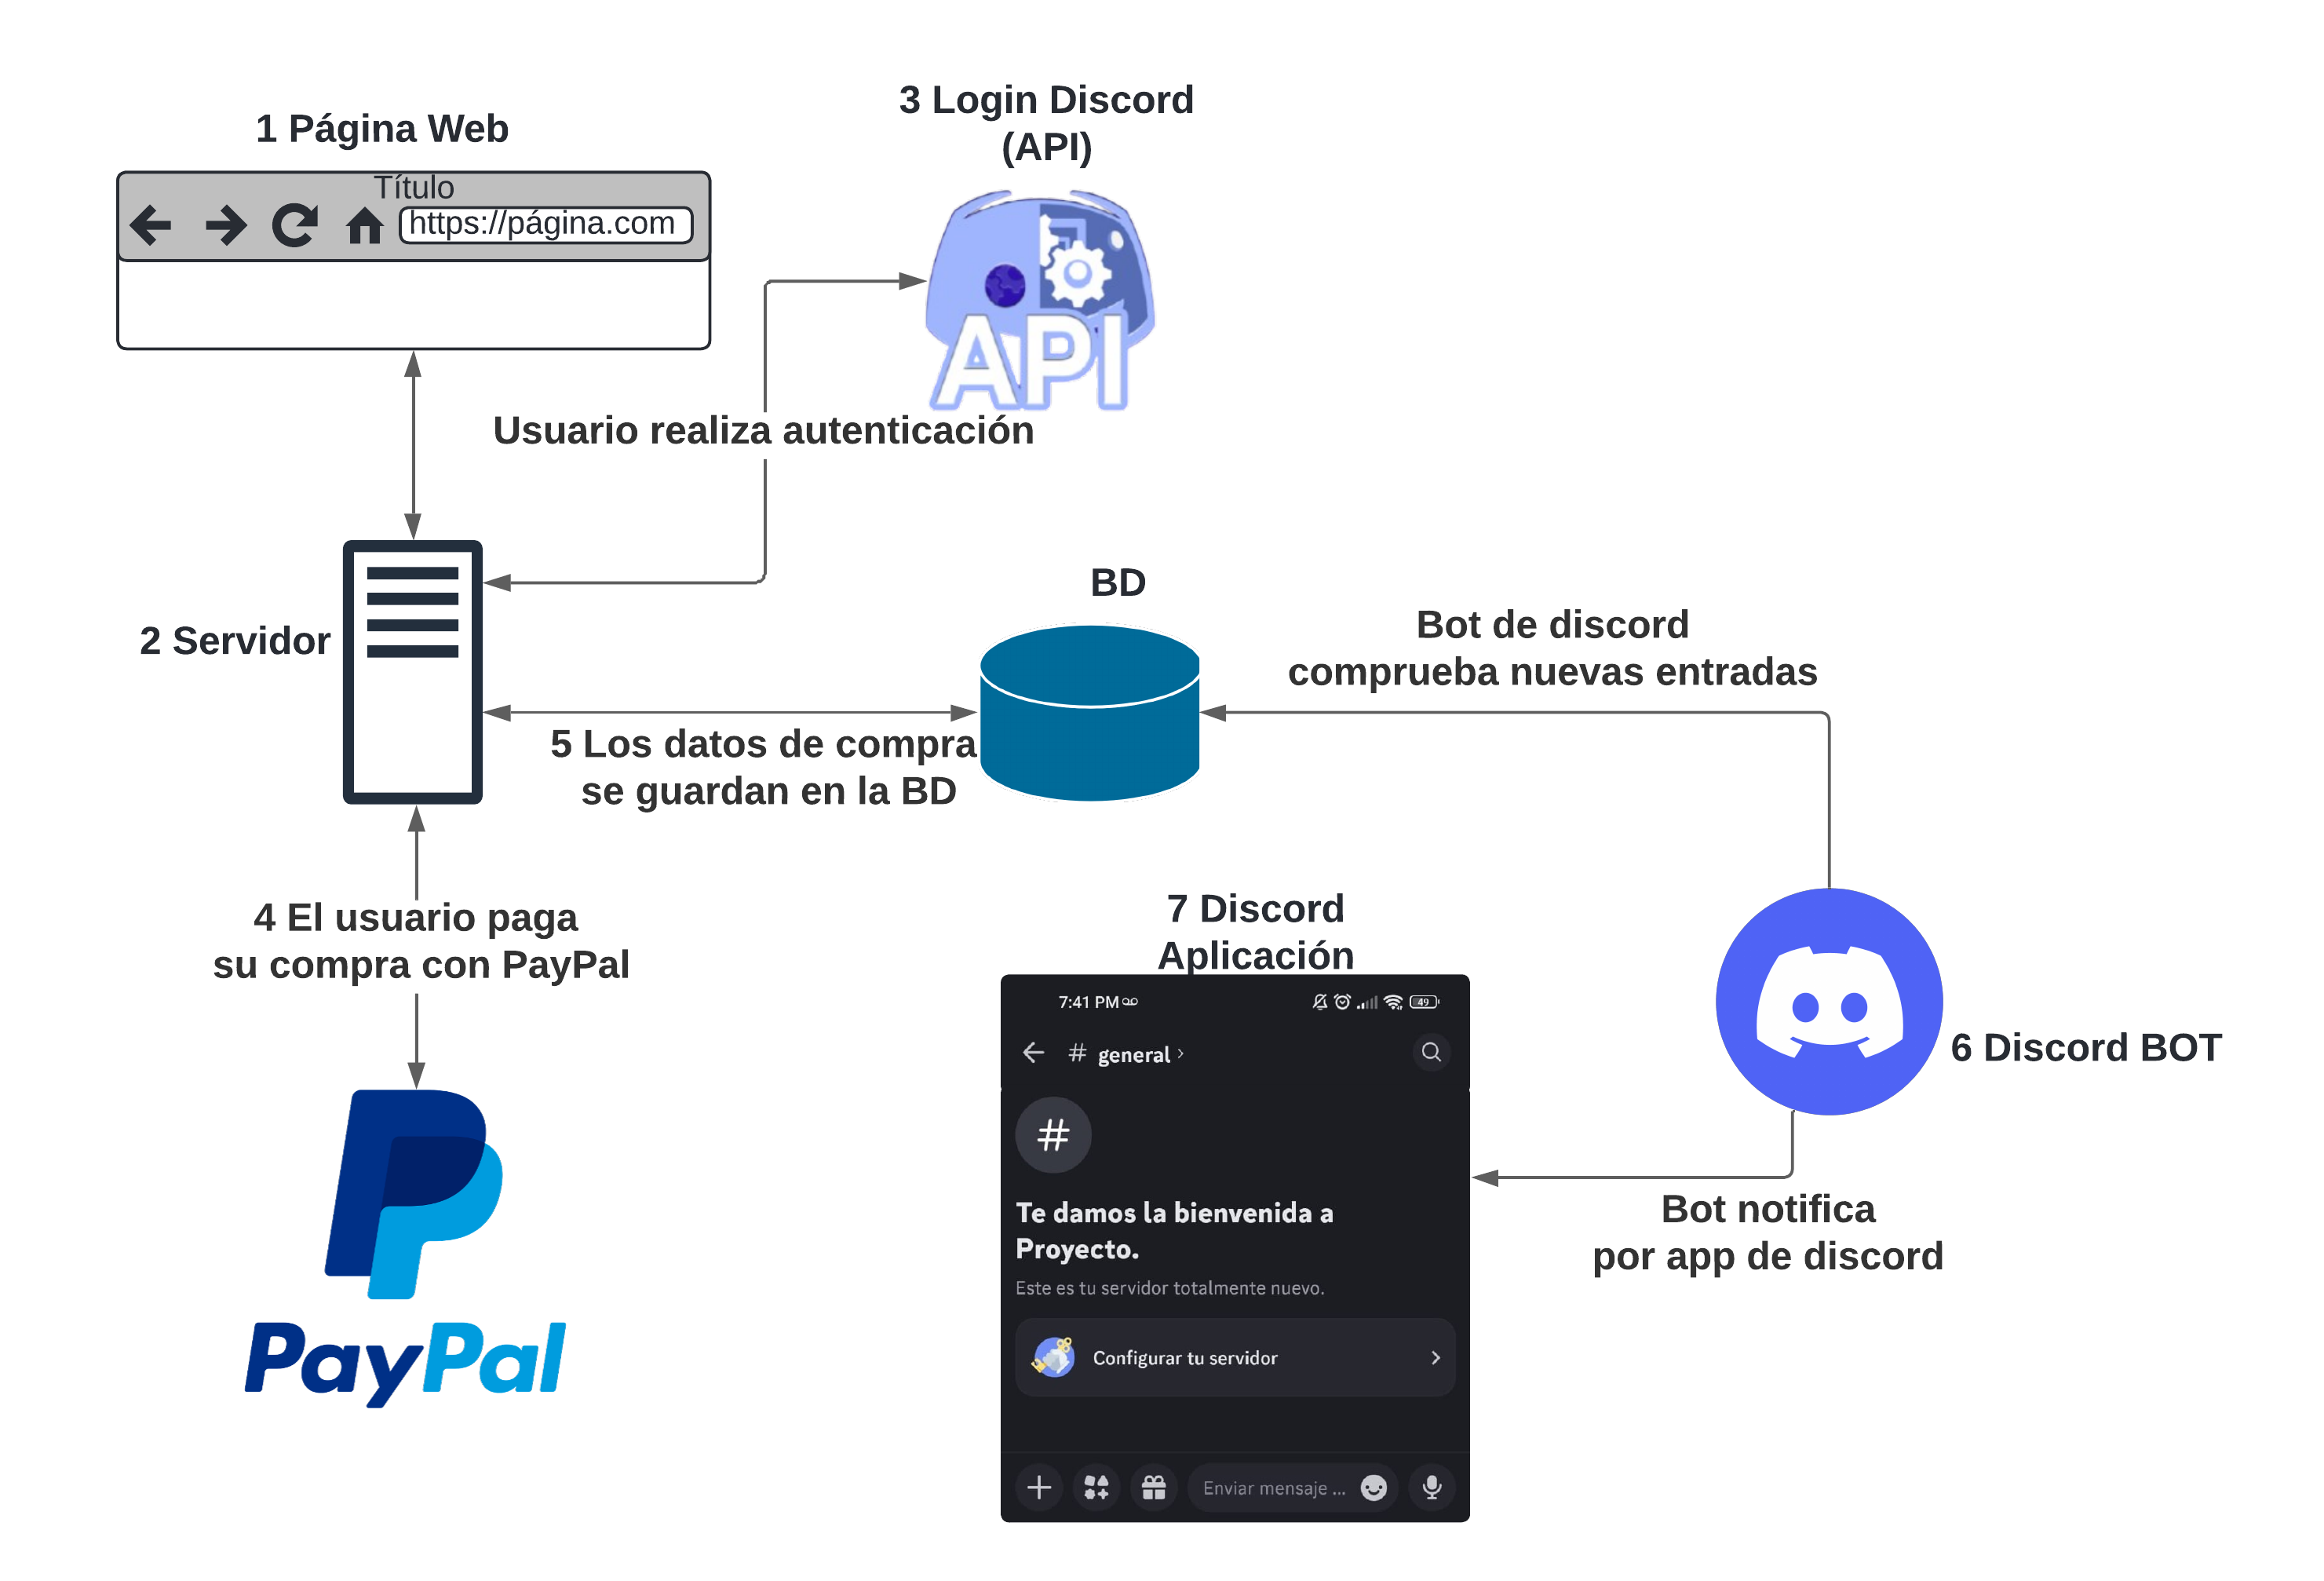
\includegraphics[width=0.8\textwidth]{./Diagramas/Diagramagen.png}
  \caption{Diagrama general del sistema}
  \label{fig:diagrama-general}
\end{figure}


\vspace{1cm}
1.- El usuario podrá consultar los artículos a la venta en el sitio web.\\

2.- El servidor será el encargado de procesar todas las solicitudes que conectarán el front-end con toda la lógica. \\

3.- El sistema autenticará al usuario mediante su cuenta de Discord.\\

4.- Una vez teniendo artículos en el carrito de compra, el usuario podrá comprarlos y pagarlos mediante PayPal; deberá realizar una autenticación dentro de PayPal para poder acceder a su cuenta y realizar el pago.\\

5.- En la base de datos se guardarán todos los datos necesarios para autenticación, los datos de compra, y los artículos que se han colocado a la venta.\\

6.- El bot de Discord hará una función administrativa, esta será avisarle al administrador y al usuario comprador sobre su compra o próximas suscripciones. Estos avisos serán personales para cada usuario.\\

7.- Mediante Discord, el usuario recibirá las notificaciones que le enviará el bot; el usuario requiere un perfil dentro de Discord.\\


\subsection{Diagramas de Secuencia}
En esta sección se presentan los diagramas de secuencia que ilustran los flujos de interacción entre los diferentes objetos durante los procesos de autenticación y compra.
\subsubsection{Diagramas de Secuencia de Autenticación y Compra}
El diagrama secuencial de autenticación y compra muestra el envío de mensajes e interacción entre los objetos durante el proceso de autenticación del usuario y la realización de una compra.
\begin{figure}[H]
  \centering
  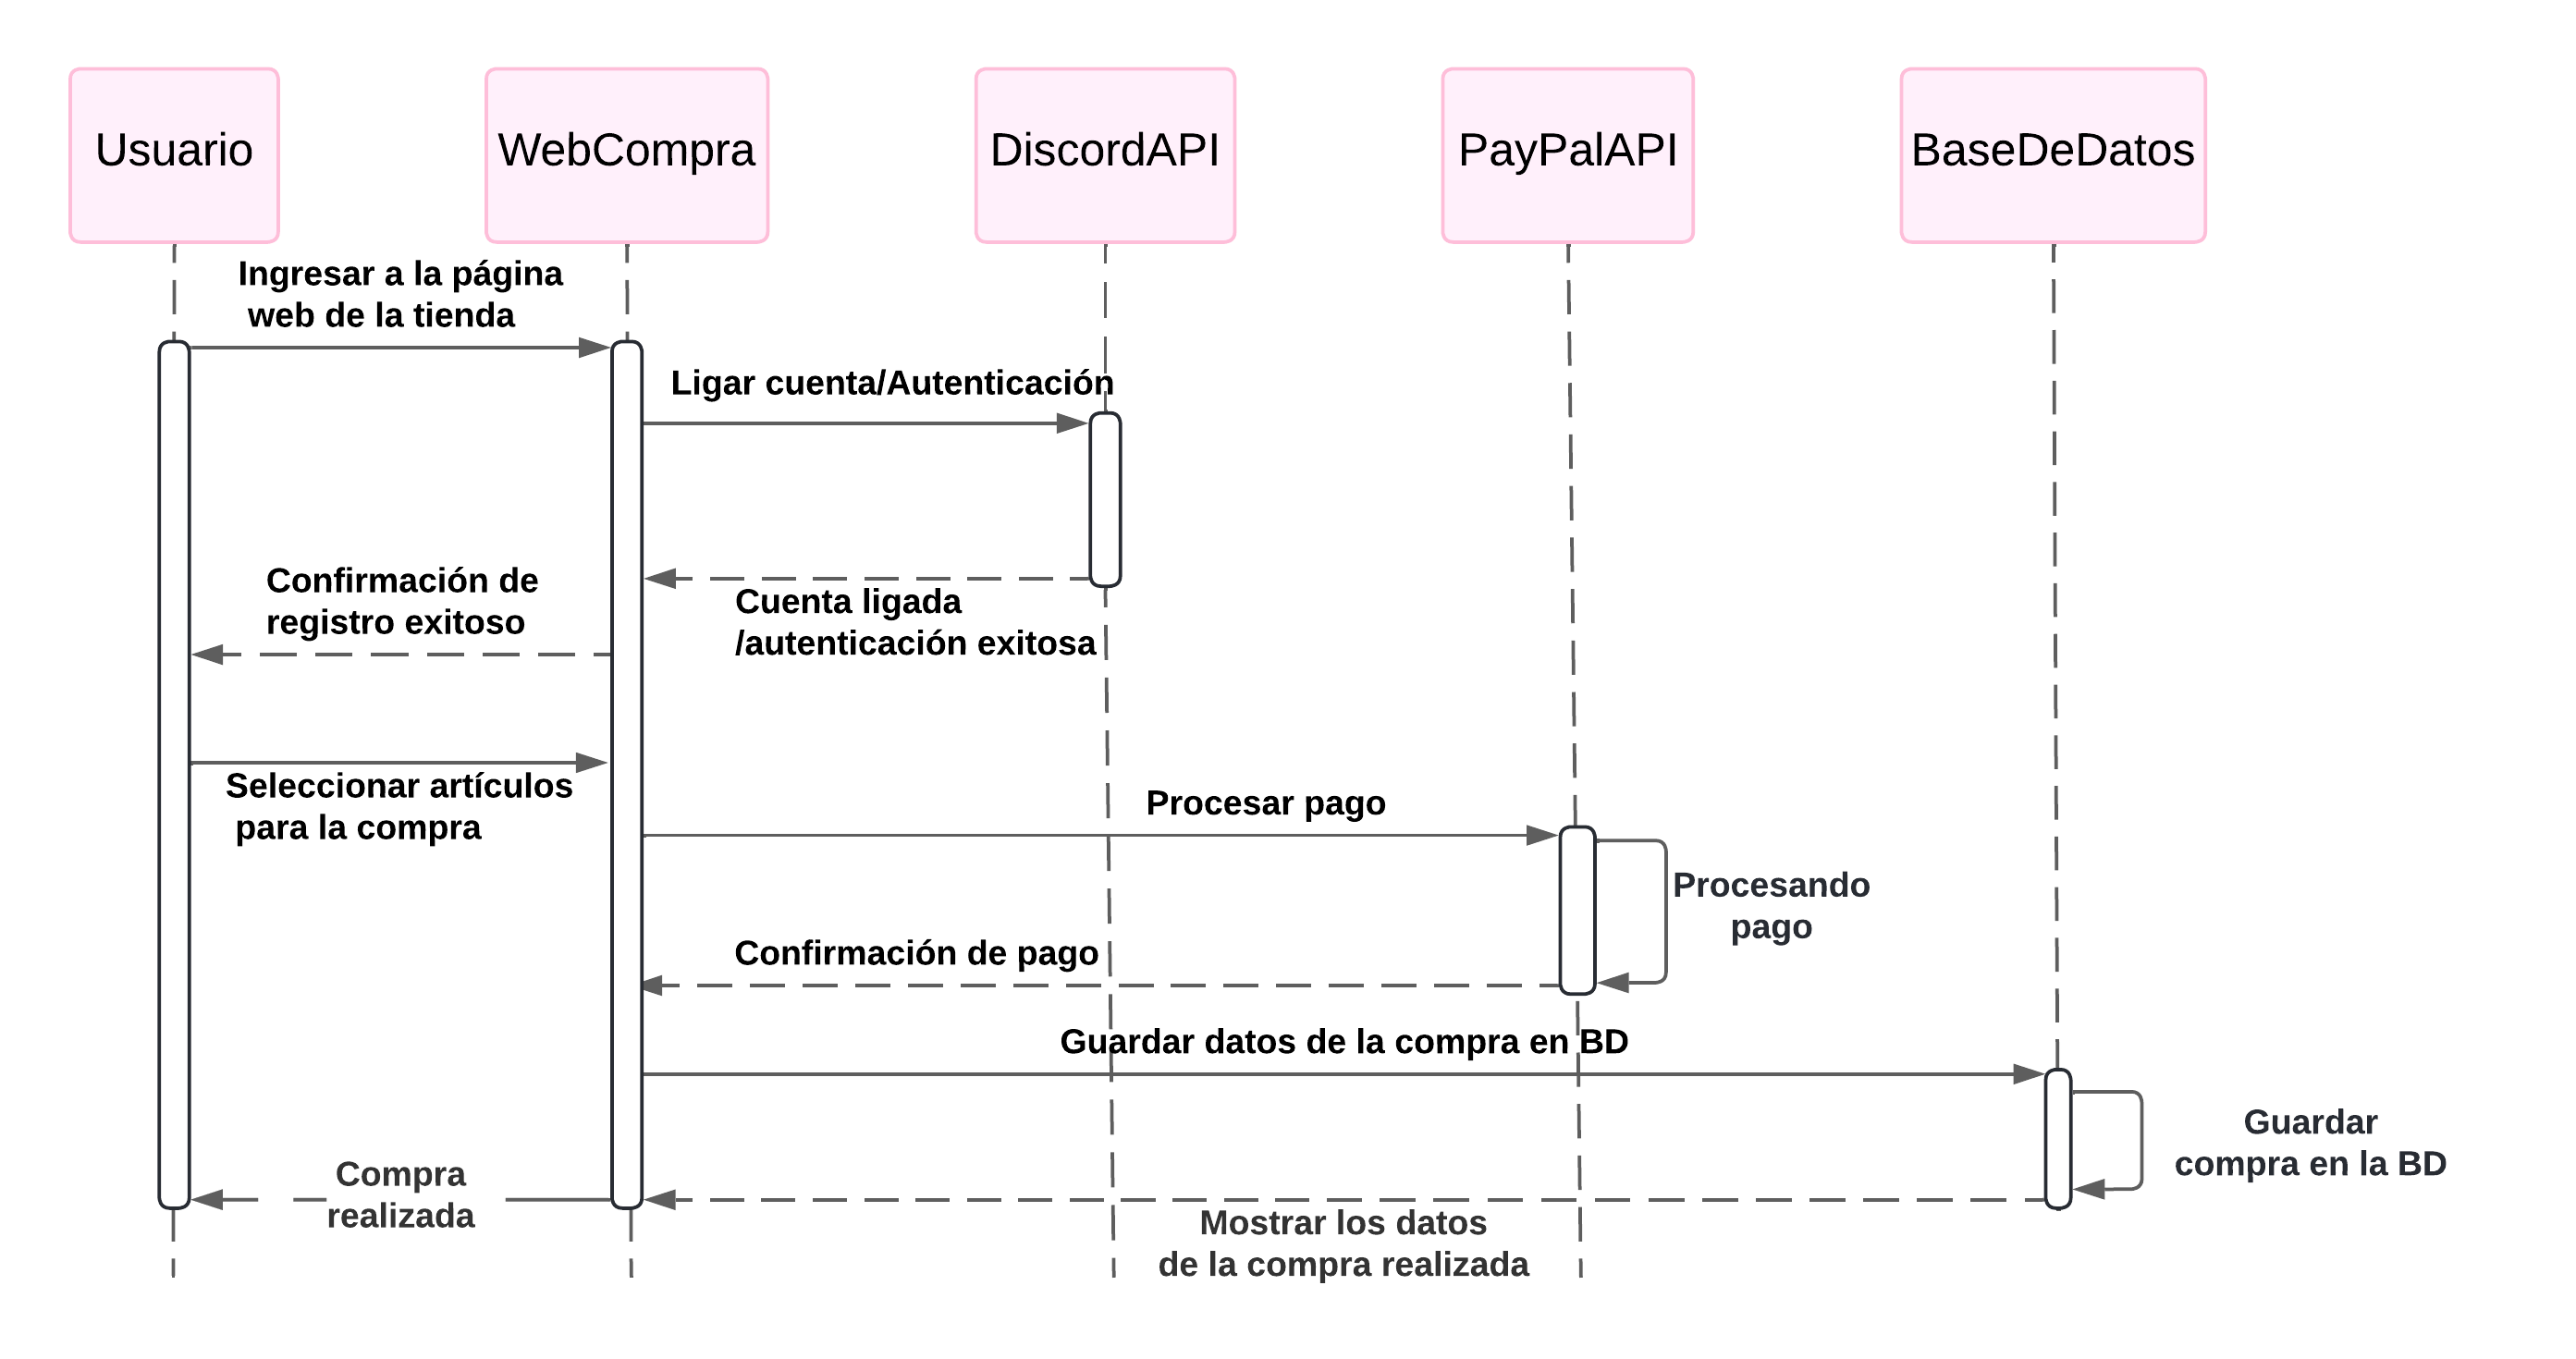
\includegraphics[width=1\textwidth]{./Diagramas/Diagramasec1.png}
  \caption{Diagrama secuencial de autenticación y compra}
  \label{fig:diagrama-secuencial1}
\end{figure}
1.- El usuario deberá iniciar sesión, autenticarse en la página web para poder realizar compras.\\

2.- Una vez seleccionado el artículo de compra, se mandará al usuario a realizar su compra; se usará PayPal para realizar la validación de compra.\\

3.- La compra realizada se registrará en la base de datos.\\

4.- Se le mostrará al usuario un mensaje de compra exitosa.
\newpage
\subsubsection{Diagramas de Secuencia de Notificación por Bot}
El diagrama secuencial de notificación por bot muestra el flujo de interacción entre los objetos durante el proceso de notificación al usuario sobre su compra.
\begin{figure}[H]
  \centering
  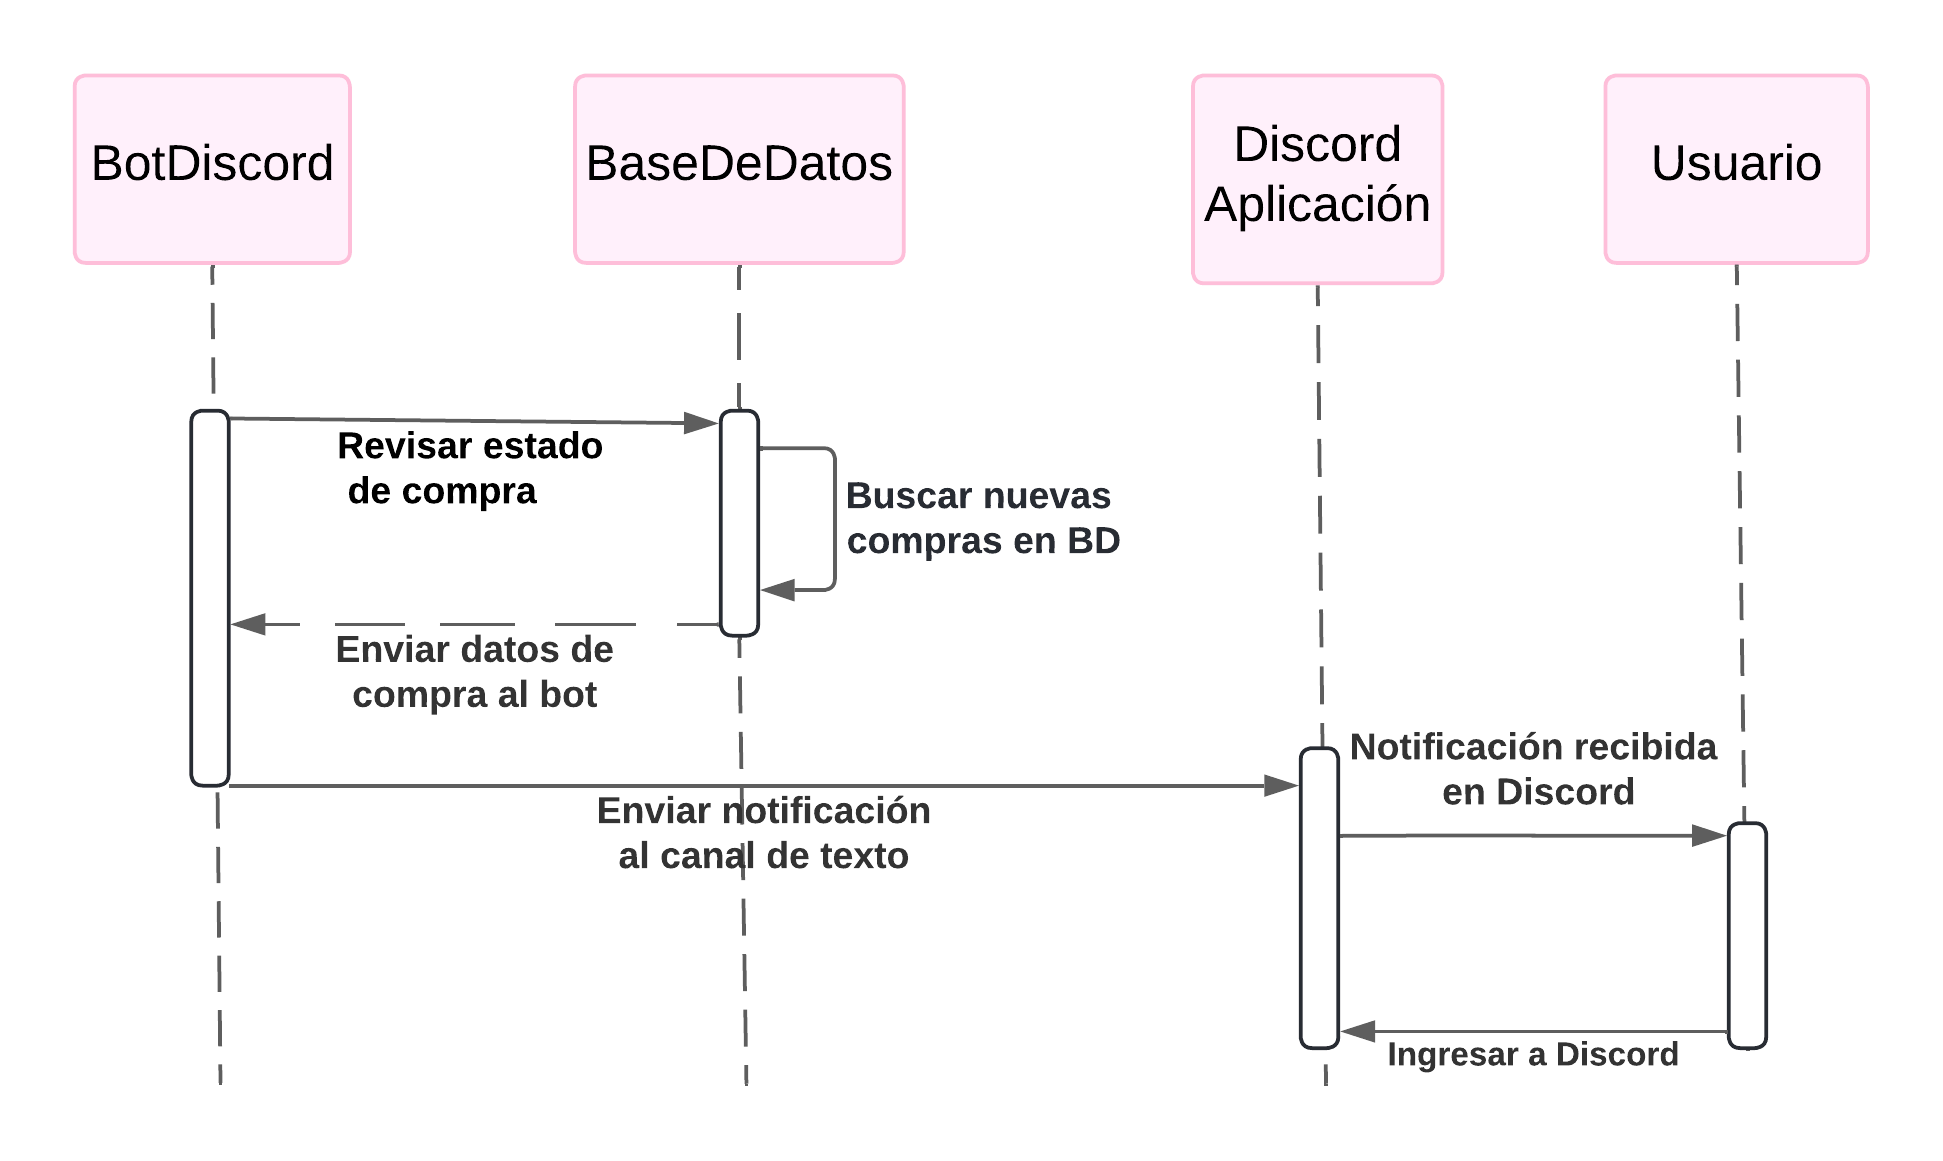
\includegraphics[width=1\textwidth]{./Diagramas/Diagramasec2.png}
  \caption{Diagrama secuencial de notificación por bot}
  \label{fig:diagrama-secuencial2}
\end{figure}

1.- El bot de Discord comprobará si hay nuevas entradas en la BD.\\

2.- El bot enviará los datos de compra vía Discord.\\

3.- El usuario comprador podrá ver los datos de su compra en el mensaje dejado por el bot.\\
\newpage

\subsection{Diagrama de la Base de Datos}
En esta sección se presenta el diseño de la base de datos, incluyendo su modelo conceptual y lógico.
\subsubsection{Modelo Conceptual de la Base de Datos}
Se presentará el modelo conceptual de la base de datos, que incluye las entidades principales y sus relaciones.
\begin{figure}[H]
  \centering
  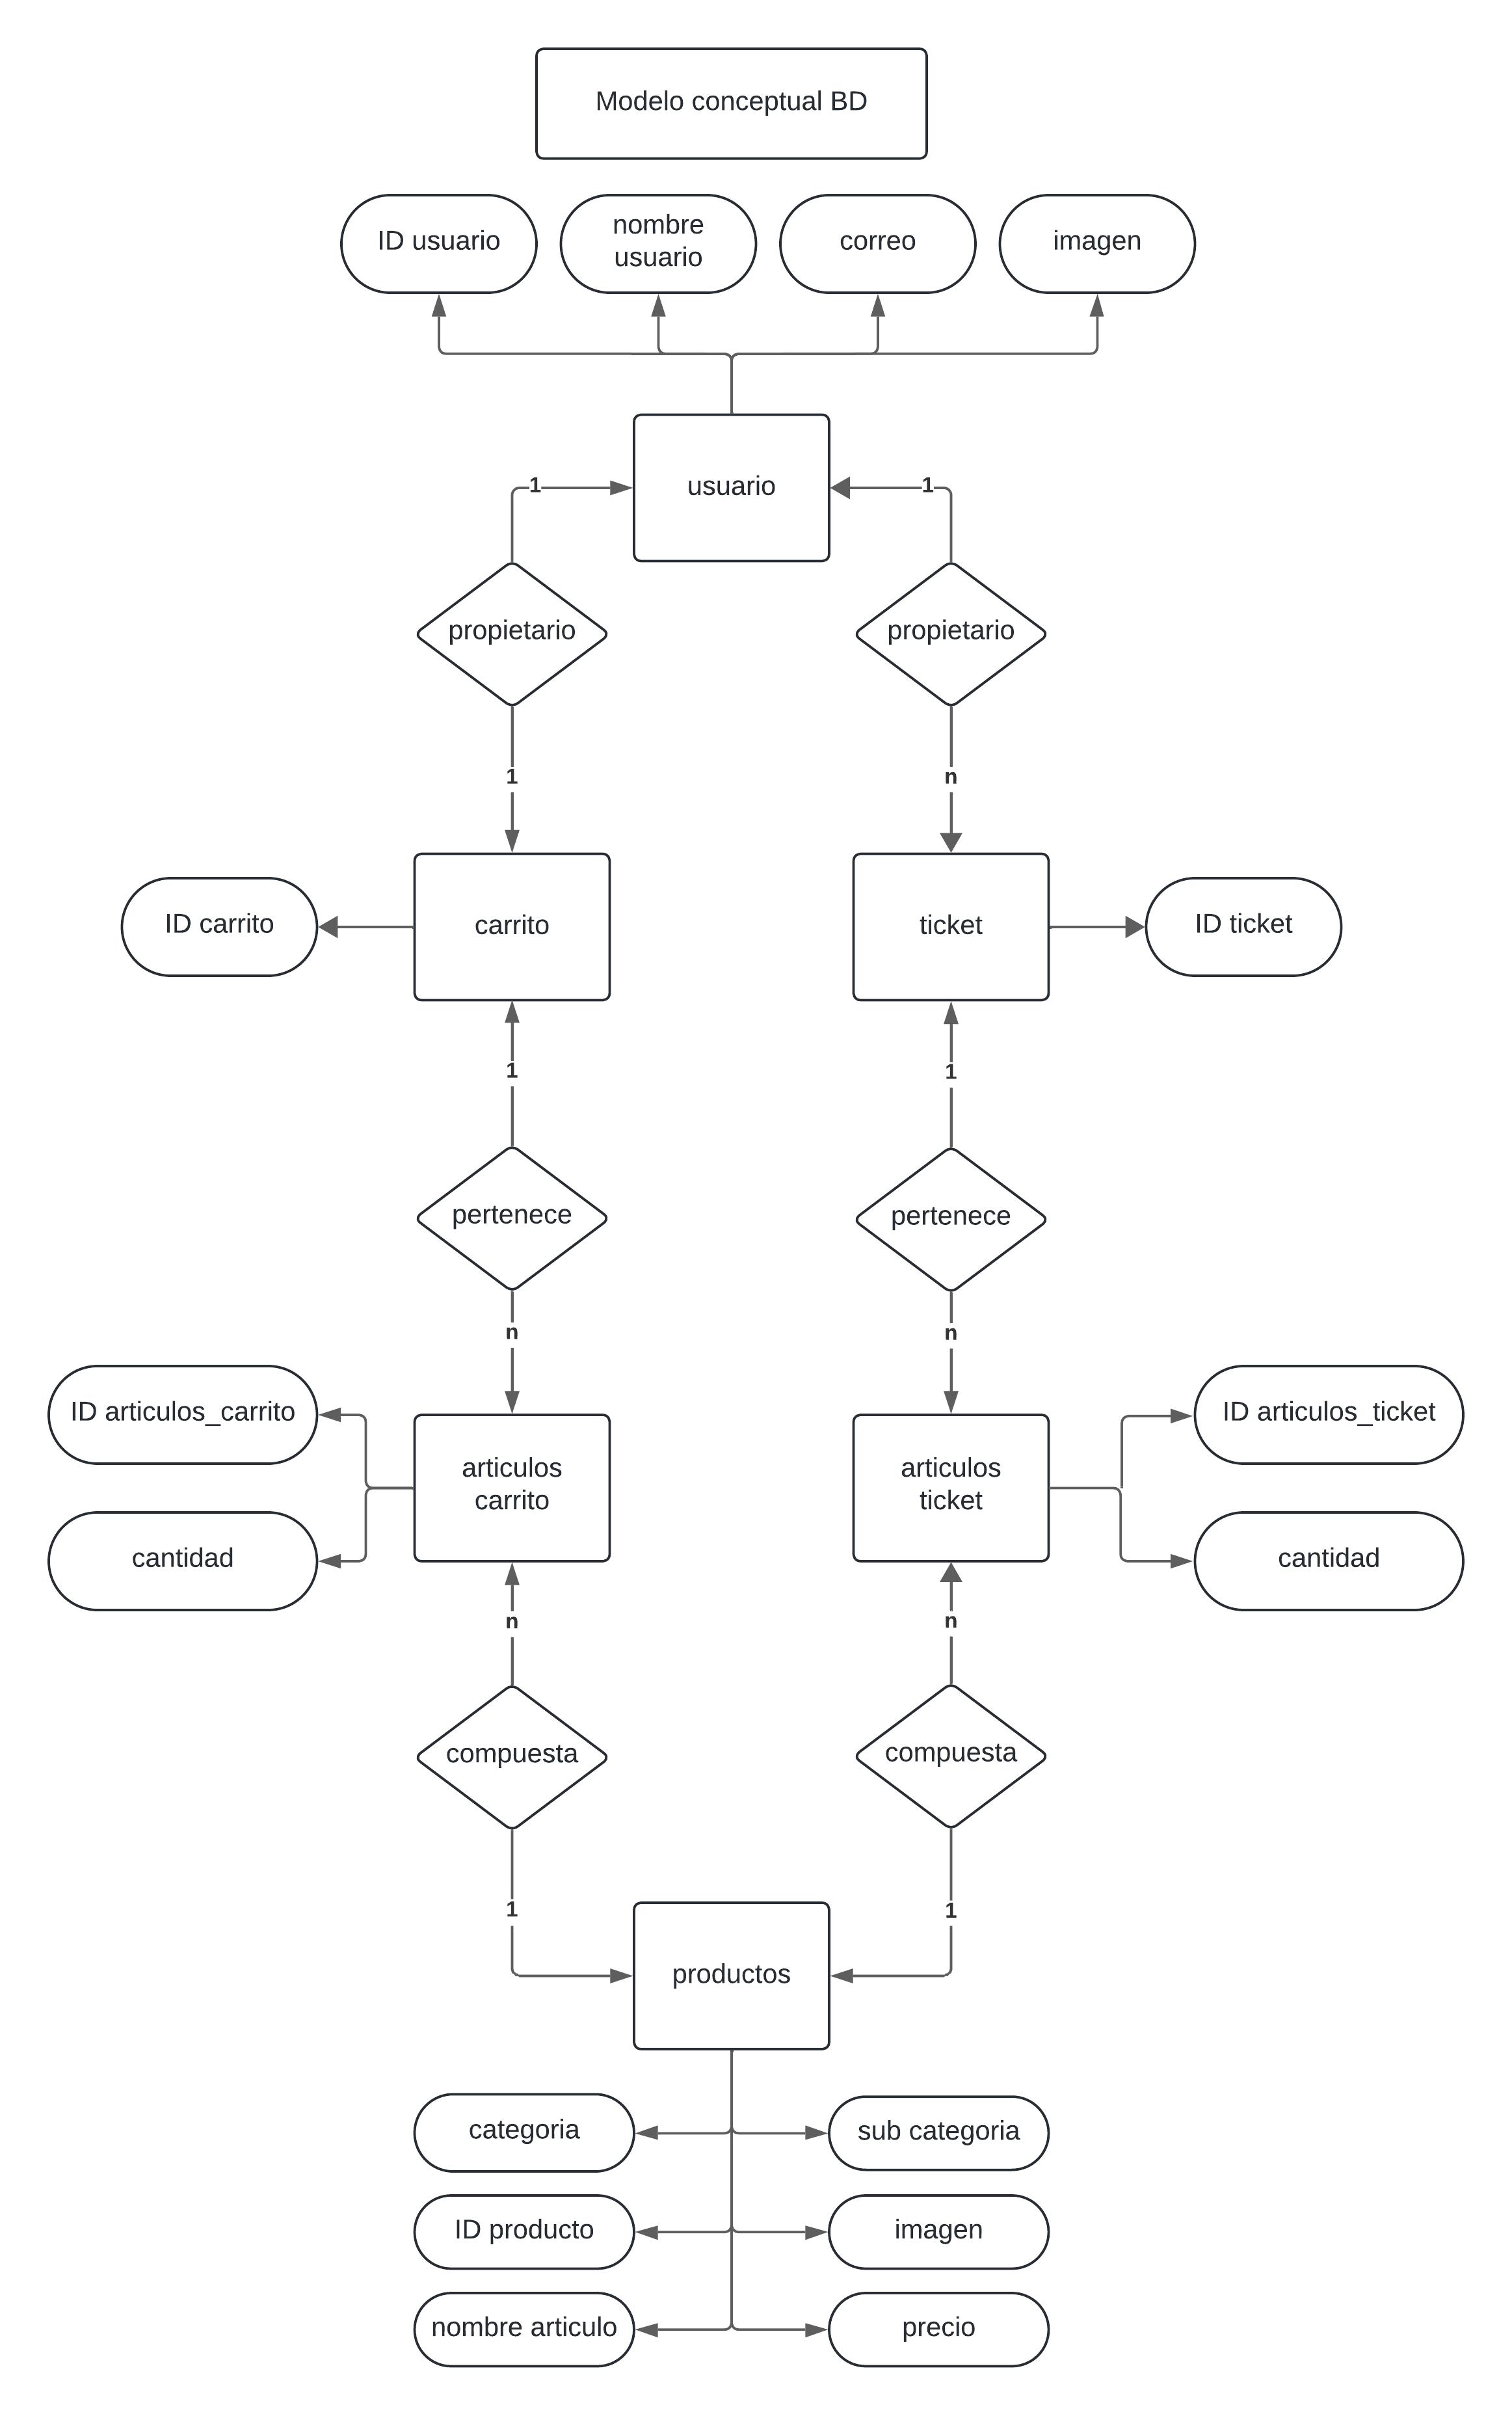
\includegraphics[width=0.5\textwidth]{./Diagramas/ModeloConsep.png}
  \caption{Modelo conceptual de la base de datos}
  \label{fig:modelo-conceptual}
\end{figure}

El diagrama de la figura~\ref{fig:modelo-conceptual} comienza con la entidad usuario, que contiene información básica como ID, nombre, correo e imagen. Cada usuario puede ser propietario de un carrito y puede tener muchos tickets, lo que implica que un mismo usuario puede realizar varias compras, pero solo tener un carrito activo a la vez.\\

El carrito está relacionado con el usuario mediante una relación de propiedad uno a uno, y contiene múltiples artículos del carrito, es decir, productos que el usuario ha agregado antes de comprar. Estos artículos tienen una cantidad y se relacionan con la entidad productos, lo cual indica qué producto específico se añadió y en qué cantidad.\\

Una vez que el usuario realiza una compra, se genera un ticket, también asociado al usuario, pero en una relación de uno a muchos (un usuario puede tener muchos tickets). El ticket contiene artículos del ticket, similares a los del carrito, con su respectiva cantidad y referencia al producto adquirido.\\

La entidad productos es el catálogo general, donde se guarda información de cada artículo como su ID, nombre, categoría, subcategoría, imagen y precio. Esta entidad es común tanto para los artículos del carrito como para los del ticket, ya que los productos son los mismos, solo cambian de estado según estén en proceso de compra (carrito) o ya comprados (ticket).\\ 
\subsubsection{Modelo Lógico de la Base de Datos}
Se presentará el modelo lógico de la base de datos, que incluye las tablas y sus relaciones así como sus atributos.
\begin{figure}[H]
  \centering
  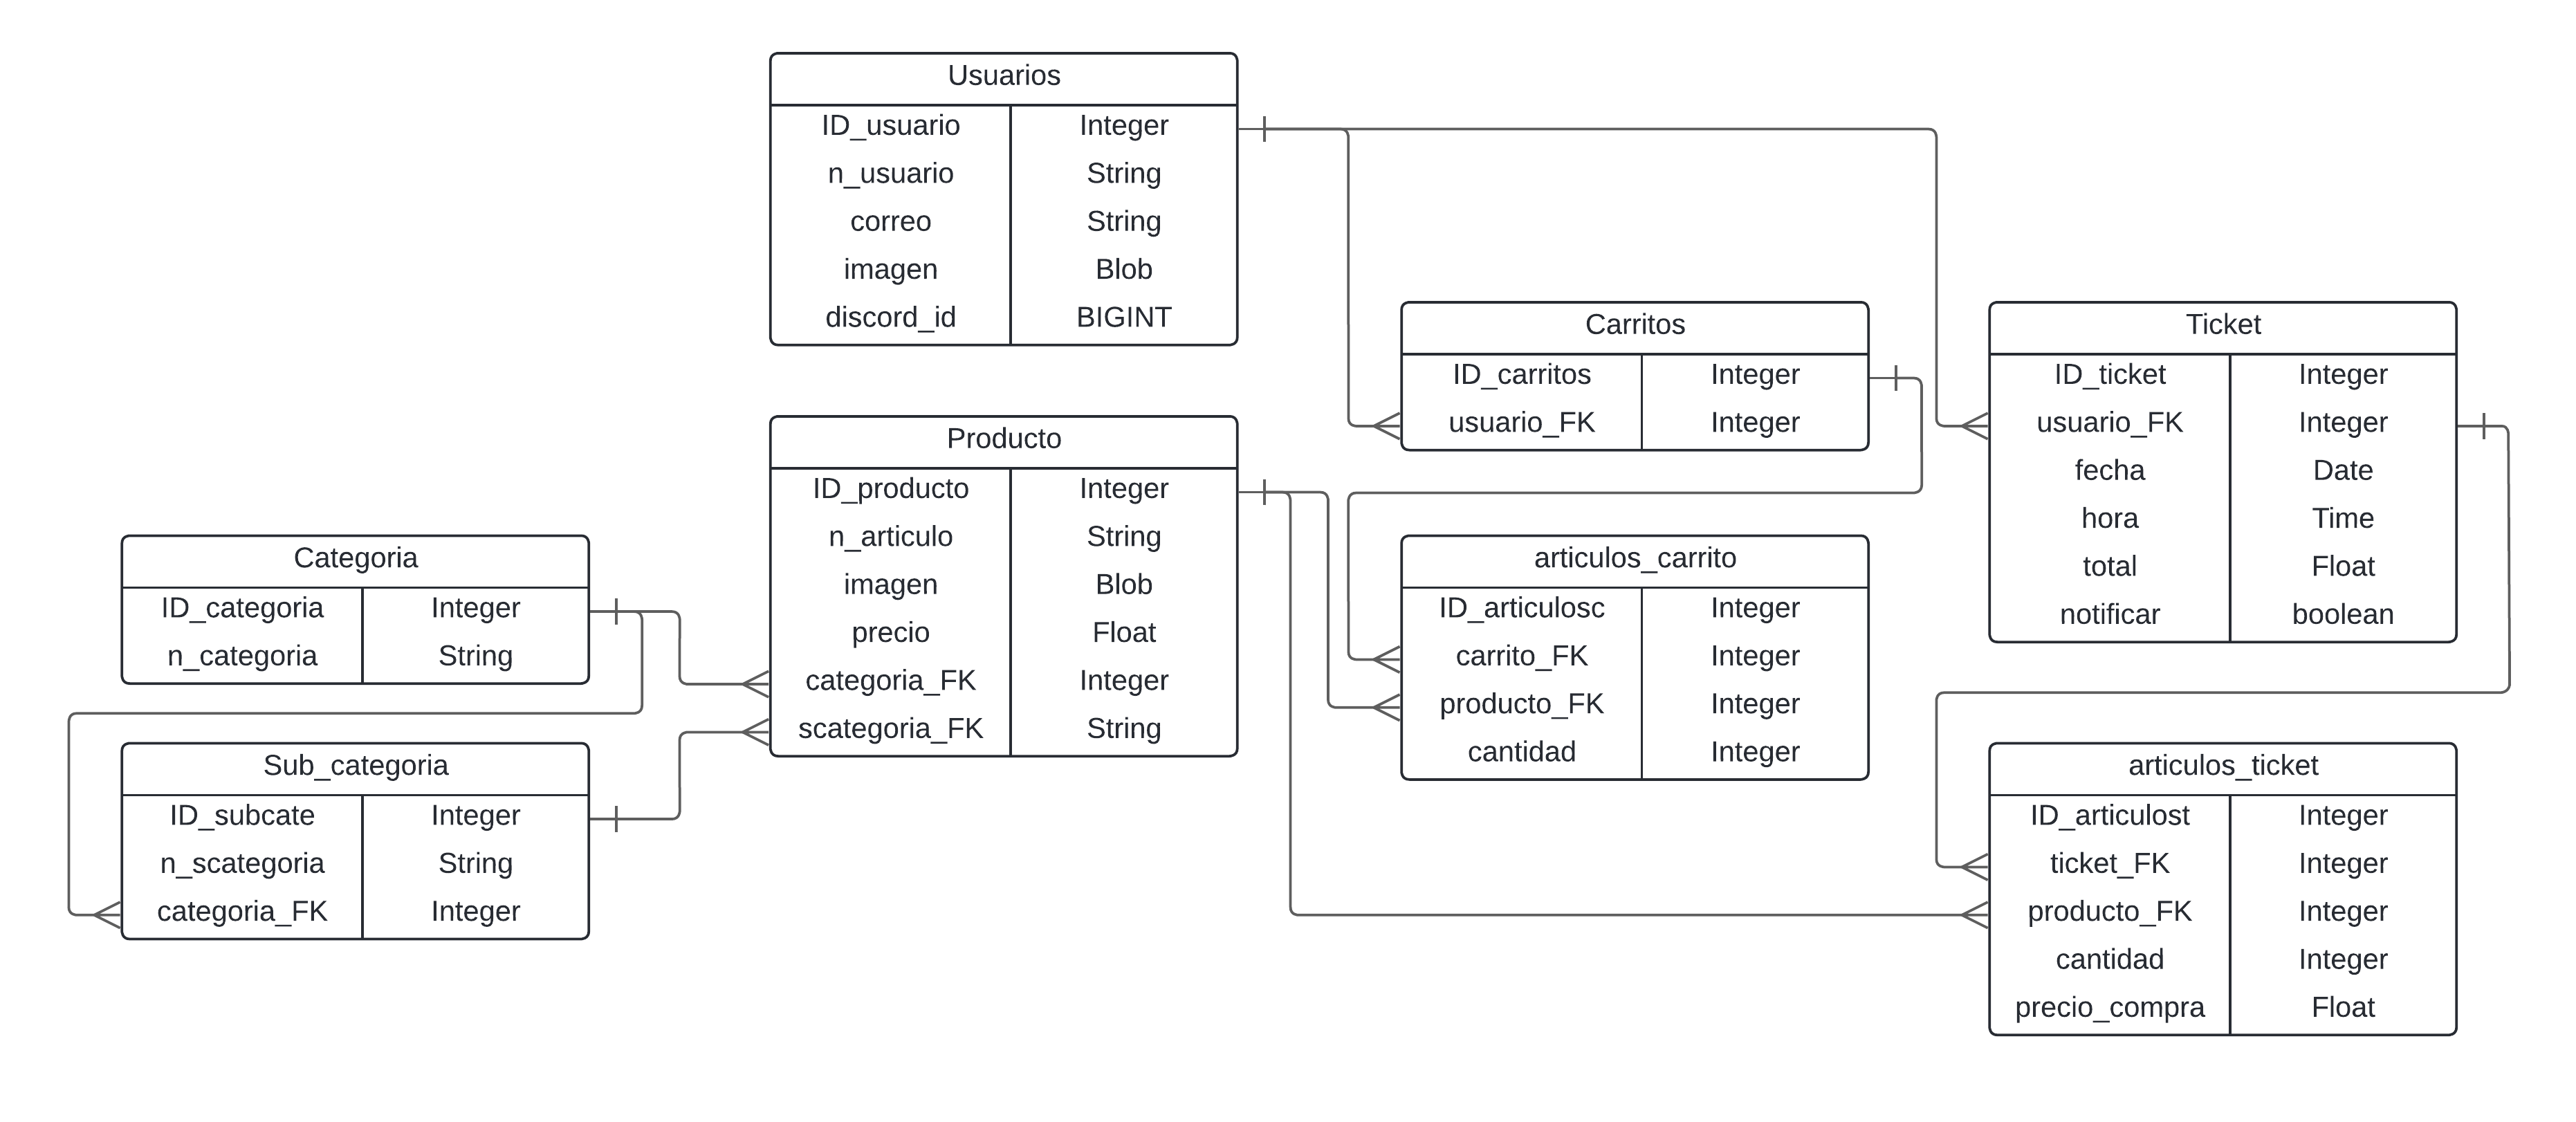
\includegraphics[width=1\textwidth]{./Diagramas/DiagramaBD.png}
  \caption{Diagrama lógico de la base de datos}
  \label{fig:diagrama-bd}
\end{figure}

En el diagrama de la figura~\ref{fig:diagrama-bd} de base de datos, la entidad Usuarios almacena la información del cliente como ID, nombre, correo e imagen. Cada usuario puede tener un carrito (relación uno a uno) y también puede generar tickets de compra (relación uno a muchos).\\

El carrito está relacionado con el usuario mediante la clave foránea \textnormal{usuario\_FK} y contiene productos a través de la tabla \textnormal{articulos\_carrito}, donde se guarda qué producto fue agregado \textnormal{producto\_FK} y en qué cantidad.\\

Cuando se realiza una compra, se genera un ticket que también pertenece a un usuario (\textnormal{usuario\_FK}) y contiene información como fecha, hora, total de la compra y si se notificó. Los productos comprados se guardan en la tabla \textnormal{articulos\_ticket}, con su cantidad y el precio al momento de la compra (\textnormal{precio\_compra}), todo enlazado al ticket (\textnormal{ticket\_FK}) y al producto (\textnormal{producto\_FK}).\\

La entidad Producto almacena todos los artículos disponibles: su ID, nombre, imagen, precio y dos claves foráneas que lo conectan con su categoría y subcategoría (\textnormal{categoria\_FK} y \textnormal{scategoria\_FK}). Las categorías están organizadas en dos niveles, mediante las tablas Categoria y \textnormal{Sub\_categoria}, esta última relacionada con la primera a través de \textnormal{categoria\_FK}.


\section{Desarrollo del sistema}
En esta sección se describen las APIs que se implementarán en el sistema, tanto internas como externas. Estas APIs son fundamentales para la comunicación entre los diferentes componentes del sistema, como la tienda en línea y el bot de Discord, facilitando el intercambio de datos de forma estructurada y segura. A través de estas interfaces, el sistema podrá recibir eventos, enviar notificaciones y ejecutar funcionalidades clave que permiten la integración fluida entre la plataforma de e-commerce y Discord.
\subsection{APIs}

En esta sección se describen las APIs que formarán parte del sistema, tanto internas como externas. Las APIs (Interfaces de Programación de Aplicaciones) permiten la comunicación entre los diferentes componentes del sistema, como la tienda en línea y el bot de Discord, facilitando el intercambio de datos de forma estructurada y segura. A través de estas interfaces, el sistema podrá recibir eventos, enviar notificaciones y ejecutar funcionalidades clave que permiten la integración fluida entre la plataforma de e-commerce y Discord.

\subsubsection{API de PayPal}

PayPal es la plataforma de pagos elegida para este proyecto debido a su facilidad de implementación, seguridad y amplia aceptación entre los usuarios. La integración se realizó utilizando el SDK oficial @paypal/checkout-server-sdk para Node.js, que proporciona métodos seguros y eficientes para procesar transacciones.\\
\newpage
\textbf{Configuración del Entorno PayPal}\\

La configuración se realizó creando un cliente PayPal dedicado que maneja la comunicación con la API. Se utilizó el entorno sandbox para desarrollo y pruebas, configurado directamente en el código:

\begin{lstlisting}[language=JavaScript, caption={Configuración del cliente PayPal}]
// Cliente PayPal SDK para procesar pagos online
const paypal = require('@paypal/checkout-server-sdk');

// Configuración del entorno PayPal en modo sandbox (desarrollo/pruebas)
const environment = new paypal.core.SandboxEnvironment(
    // Client ID de PayPal para aplicacion sandbox
    'AW4xEijNfSBJiSYtmQn0f_ABCdasd1-dNdjmw_XZ2fIDPrbvqZQZBSy4fQn',
    // Client Secret de PayPal (CONFIDENCIAL - para autenticación del servidor)
    'EHImBnGza7Csas8CsdscAKHfbHV9s8SNOk39YW9L5A9B_fISZwPPP'
);

// Cliente HTTP configurado para comunicarse con la API de PayPal
const client = new paypal.core.PayPalHttpClient(environment);

module.exports = client;
\end{lstlisting}

\textbf{Implementación del Flujo de Pago}\\

El proceso de pago se divide en dos etapas principales: la creación de la orden en el frontend y la captura del pago en el backend. Este flujo garantiza la seguridad de la transacción y permite verificar el estado del pago antes de procesar la compra.\\

\textbf{Etapa 1: Creación de la Orden (Frontend)}\\

En el frontend, se utiliza el componente PayPalButtons de la librería @paypal/react-paypal-js. Este componente maneja automáticamente la interfaz de usuario y la comunicación inicial con PayPal:
\newpage
\begin{lstlisting}[language=JavaScript, caption={Implementación del botón PayPal en React}]
// Configuración inicial del SDK de PayPal
const initialOptions = {
    "client-id": "AW4xEijNfSBJiSYtmQn0f_ABCdasd1-dNdjmw_XZ2fIDPrbvqZQZBSy4fQn",
    currency: "MXN", // Moneda mexicana
};

<PayPalButtons
    style={{ layout: "vertical" }}
    // Función que se ejecuta al crear la orden de pago
    createOrder={(data, actions) => {
        return actions.order.create({
            purchase_units: [
                {
                    amount: {
                        value: total.toFixed(2),
                    },
                },
            ],
        });
    }}
    // Función que se ejecuta cuando PayPal aprueba el pago
    onApprove={async (data, actions) => {
        try {
            const totalFloat = parseFloat(total);
            
            // Enviar datos de la orden al backend para completar el pago
            const response = await fetch(`${process.env.REACT_APP_BACKEND_URL}/api/paypal/capture-order`, {
                method: 'POST',
                headers: {
                    'Content-Type': 'application/json',
                },
                credentials: 'include', // Incluir cookies de autenticación
                body: JSON.stringify({ orderId: data.orderID, total: totalFloat }),
            });

            if (response.ok) {
                // Pago exitoso - mostrar mensaje y recargar pagina
                setPopupMessage('Pago completado exitosamente');
                window.location.reload();
            }
        } catch (error) {
            console.error('Error al capturar el pago:', error);
        }
    }}
/>
\end{lstlisting}
\newpage
\textbf{Etapa 2: Captura del Pago (Backend)}\\

Una vez que el usuario aprueba el pago en la interfaz de PayPal, el frontend envía el ID de la orden al backend para completar la captura usando el SDK de PayPal:

\begin{lstlisting}[language=JavaScript, caption={Captura de orden PayPal en el backend}]
// Ruta para capturar una orden de PayPal y procesar la compra
router.post('/capture-order', async (req, res) => {
    const { orderId, total } = req.body;

    // Crear solicitud de captura usando el SDK de PayPal
    const request = new paypal.orders.OrdersCaptureRequest(orderId);
    request.requestBody({}); // Cuerpo vacio para captura simple

    try {
        // Ejecutar la captura de la orden en PayPal usando su API
        const capture = await client.execute(request);
        const order = capture.result;

        // Verificar que el pago se completo exitosamente en PayPal
        if (order.status === 'COMPLETED') {
            // Obtener informacion del usuario desde las cookies
            const userCookie = req.cookies.user;
            const user = JSON.parse(userCookie);
            const discordId = user.id;

            // Buscar el ID del usuario en la base de datos
            const [rows] = await pool.query('SELECT ID_usuarios FROM usuarios WHERE discord_id = ?', [discordId]);
            const userId = rows[0].ID_usuarios;

            // Crear el ticket de compra usando el modelo Ticket
            const ticketId = await Ticket.create(userId, total);

            res.json({ success: true, message: 'Pago completado exitosamente y ticket creado.', ticketId });
        } else {
            res.status(400).json({ success: false, message: 'El pago no se completó.' });
        }
    } catch (error) {
        console.error('Error al capturar el pago:', error);
        res.status(500).json({ success: false, message: 'Error al capturar el pago.' });
    }
});
\end{lstlisting}

Este flujo de dos etapas permite que PayPal maneje toda la complejidad de la autenticación del usuario, la validación de métodos de pago y el procesamiento seguro de la transacción, mientras que el backend se encarga de confirmar y registrar la compra una vez completada. Una ventaja clave de PayPal es su entorno sandbox que permite realizar pruebas completas sin manejar dinero real, verificando que la integración funciona correctamente antes del despliegue en producción.\\

\subsubsection{API de Discord OAuth2}

La implementación de Discord OAuth2 permite a los usuarios autenticarse utilizando sus credenciales de Discord, eliminando la necesidad de crear cuentas adicionales.\\

\textbf{Configuración de la Aplicación Discord}\\

Para implementar OAuth2 con Discord, primero se registró una aplicación en el Portal de Desarrolladores de Discord. En el backend, se configuró un controlador de autenticación que centraliza todas las operaciones OAuth2:

\begin{lstlisting}[language=JavaScript, caption={Configuración del controlador de autenticación Discord}]
class AuthController {
    constructor() {
        // Configuracion de endpoints de Discord API
        this.discordOAuth2URL = 'https://discord.com/api/oauth2/authorize';
        this.tokenURL = 'https://discord.com/api/oauth2/token';
        this.userInfoURL = 'https://discord.com/api/users/@me';
        this.redirectURI = process.env.DISCORD_REDIRECT_URI;
        this.clientID = process.env.DISCORD_CLIENT_ID;
        this.clientSecret = process.env.DISCORD_CLIENT_SECRET;
    }
}
\end{lstlisting}

\textbf{Flujo de Autenticación OAuth2}\\

El proceso OAuth2 de Discord sigue un flujo estándar de autorización que se divide en varias etapas claramente definidas:

\textbf{Etapa 1: Inicio del Flujo de Autorización}\\

Cuando el usuario hace clic en Iniciar sesión con Discord, el backend genera una URL de autorización y redirigirá al usuario a Discord:

\begin{lstlisting}[language=JavaScript, caption={Inicio del flujo OAuth2}]
login(req, res) {
    const scope = 'identify email'; // Permisos solicitados a Discord
    const state = crypto.randomBytes(16).toString('hex'); // Token anti-CSRF
    
    // Guardar estado en cookie temporal para validacion posterior
    res.cookie('oauth_state', state, { 
        httpOnly: true, 
        maxAge: 60000, // 1 minuto de expiracion
        sameSite: 'lax'
    });

    // Construir URL de autorizacion Discord
    const url = `${this.discordOAuth2URL}?client_id=${this.clientID}&redirect_uri=${encodeURIComponent(this.redirectURI)}&response_type=code&scope=${encodeURIComponent(scope)}&state=${state}`;
    res.redirect(url);
}
\end{lstlisting}

En esta etapa, el sistema genera un token `state` aleatorio que se almacena temporalmente en una cookie para prevenir ataques CSRF (Cross-Site Request Forgery). Discord requiere los permisos `identify` y `email` para obtener información básica del usuario.\\

\textbf{Etapa 2: Autorización del Usuario en Discord}\\

Discord presenta al usuario una pantalla de autorización donde debe aprobar los permisos solicitados. Una vez autorizado, Discord redirige al usuario de vuelta a la aplicación con un código de autorización temporal.\\

La imagen de la interfaz se mostrará más adelante figura~\ref{fig:login2}.\\

\textbf{Etapa 3: Intercambio de Código por Token de Acceso}\\

El callback del backend procesa la respuesta de Discord, valida el estado e intercambia el código de autorización por un token de acceso:

\begin{lstlisting}[language=JavaScript, caption={Callback OAuth2 - Intercambio de token}]
async callback(req, res) {
    const { code, state } = req.query;
    const savedState = req.cookies.oauth_state;

    // Verificar estado para prevenir ataques CSRF
    if (!code || !state || state !== savedState) {
        return res.status(400).redirect(`${process.env.FRONTEND_URL}/`);
    }

    try {
        // Intercambiar codigo de autorizacion por token de acceso
        const tokenResponse = await axios.post(this.tokenURL, new URLSearchParams({
            client_id: this.clientID,
            client_secret: this.clientSecret,
            grant_type: 'authorization_code',
            code,
            redirect_uri: this.redirectURI,
        }), {
            headers: {
                'Content-Type': 'application/x-www-form-urlencoded',
            },
        });

        const accessToken = tokenResponse.data.access_token;
\end{lstlisting}
\newpage
\textbf{Etapa 4: Obtención de Datos del Usuario}\\

Con el token de acceso, el sistema consulta la API de Discord para obtener la información del usuario:

\begin{lstlisting}[language=JavaScript, caption={Obtención de datos del usuario desde Discord}]
        // Obtener informacion del usuario desde Discord
        const userResponse = await axios.get(this.userInfoURL, {
            headers: {
                Authorization: `Bearer ${accessToken}`,
            },
        });

        const userData = userResponse.data;
        
        // Buscar o crear usuario en la base de datos local
        const [rows] = await pool.query('SELECT * FROM usuarios WHERE discord_id = ?', [userData.id]);

        if (rows.length === 0) {
            // Insertar nuevo usuario
            await pool.query(
                'INSERT INTO usuarios (discord_id, correo, imagen, n_usuario) VALUES (?, ?, ?, ?)',
                [userData.id, userData.email, userData.avatar, userData.username]
            );
        } else {
            // Actualizar datos del usuario existente
            await pool.query(
                'UPDATE usuarios SET correo = ?, imagen = ?, n_usuario = ? WHERE discord_id = ?',
                [userData.email, userData.avatar, userData.username, userData.id]
            );
        }
\end{lstlisting}
\newpage
\textbf{Etapa 5: Creación de Sesión Mediante Cookie}\\

Finalmente, el sistema crea una cookie de sesión segura que contiene los datos esenciales del usuario:
\begin{lstlisting}[language=JavaScript, caption={Creación de cookie de sesión}]
        // Preparar datos del usuario para la cookie de sesion
        const userPayload = {
            id: userData.id,
            username: userData.global_name || userData.username,
            // Construir URL de avatar usando Discord CDN
            avatar: userData.avatar
                ? `https://cdn.discordapp.com/avatars/${userData.id}/${userData.avatar}.png`
                : `https://cdn.discordapp.com/embed/avatars/${userData.discriminator % 5}.png`,
            email: userData.email,
        };
        
        // Crear cookie de sesion con datos del usuario
        res.cookie('user', JSON.stringify(userPayload), { 
            httpOnly: true,    // Solo accesible desde el servidor (seguridad)
            secure: false,     // Para desarrollo local (HTTPS en produccion)
            maxAge: 24 * 60 * 60 * 1000, // 24 horas de duracion
            sameSite: 'lax'    // Proteccion contra CSRF
        });
        
        // Redirigir al frontend tras autenticacion exitosa
        res.redirect(`${process.env.FRONTEND_URL}/`);
    } catch (error) {
        console.error('Error during Discord authentication:', error);
        res.redirect(`${process.env.FRONTEND_URL}/`);
    }
}
\end{lstlisting}

\textbf{Gestión de Sesiones Mediante Cookies}\\

El sistema utiliza cookies HTTP para mantener la sesión del usuario autenticado. La cookie `user` contiene información esencial en formato JSON y se configura con las siguientes características de seguridad:

- \textbf{httpOnly}: La cookie solo es accesible desde el servidor, no desde JavaScript del cliente, protegiendo contra ataques XSS.

- \textbf{sameSite}: Configurada como 'lax' para protección básica contra CSRF.

- \textbf{maxAge}: Duración de 24 horas, después de las cuales el usuario debe autenticarse nuevamente.

- \textbf{secure}: Deshabilitado para desarrollo local, debe habilitarse en producción con HTTPS.

\newpage
La estructura de la cookie de usuario contiene:

\begin{lstlisting}[language=JavaScript, caption={Estructura de la cookie de sesión}]
{
  "id": "discord_user_id",           // ID unico del usuario en Discord
  "username": "nombre_usuario",       // Nombre de usuario o nombre global
  "avatar": "https://cdn.discordapp.com/avatars/...", // URL del avatar
  "email": "usuario@email.com"       // Correo electronico del usuario
}
\end{lstlisting}

\textbf{Verificación de Sesión}\\

Para operaciones posteriores, el sistema verifica la autenticación leyendo la cookie del usuario:

\begin{lstlisting}[language=JavaScript, caption={Verificación de usuario autenticado}]
// Ruta para obtener informacion del usuario autenticado
router.get('/user', (req, res) => {
    const userCookie = req.cookies.user;
    if (!userCookie) {
        return res.status(401).send('Not authenticated');
    }

    try {
        const user = JSON.parse(userCookie);
        res.json(user); // Devolver datos del usuario autenticado
    } catch (error) {
        res.status(400).send('Invalid cookie format');
    }
});
\end{lstlisting}
Implementar el inicio de sesión por medio de Discord nos permite evitar registro de usuarios y almacenamiento de contraseñas dejando la seguridad para comprobar la identidad del usuario a Discord.

\subsection{Forma Física de la Base de datos}
A continuación se explicarán algunas de las tablas principales utilizadas en este programa\footnote{Para ver toda la base de datos física así como su implementación completa, favor de visitar el repositorio del proyecto en GitHub: \url{https://github.com/Alvaro9669/PT.git}}.

\subsubsection{Tabla ticket}

La tabla \texttt{ticket} es fundamental para el sistema de notificaciones automatizadas del bot de Discord. Esta tabla almacena la información principal de cada compra realizada en la tienda:
\newpage
\begin{lstlisting}[language=SQL, caption={Estructura de la tabla ticket}]
CREATE TABLE ticket (
  ID_ticket int NOT NULL AUTO_INCREMENT,
  usuario_FK int DEFAULT NULL,
  fecha date NOT NULL,
  hora time NOT NULL,
  total float NOT NULL,
  notificar tinyint(1) DEFAULT '0',
  PRIMARY KEY (ID_ticket),
  KEY usuario_FK (usuario_FK),
  CONSTRAINT ticket_ibfk_1 FOREIGN KEY (usuario_FK) REFERENCES usuarios (ID_usuarios) ON DELETE CASCADE,
  CONSTRAINT ticket_chk_1 CHECK ((total >= 0))
) ENGINE=InnoDB AUTO_INCREMENT=53 DEFAULT CHARSET=utf8mb4 COLLATE=utf8mb4_0900_ai_ci
\end{lstlisting}

El campo más importante para el funcionamiento del bot es \texttt{notificar}, un campo booleano que actúa como un sistema de persistencia para las notificaciones pendientes. Este campo se inicializa con valor \texttt{1} (true) cuando se crea un nuevo ticket tras una compra exitosa.\\

El bot de Discord consulta periódicamente esta tabla buscando tickets donde \texttt{notificar = 1}, indicando que aún no han sido notificados al usuario. Una vez que el bot envía exitosamente la notificación por mensaje directo, actualiza este campo a \texttt{0} (falso), marcando el ticket como ya notificado.\\

Esta implementación garantiza que, incluso si el bot se reinicia o experimenta fallos temporales, mantenga un registro persistente de qué tickets faltan por notificar. De esta manera, ninguna compra queda sin su respectiva notificación, funcionando como una cola de notificaciones pendientes con persistencia en la base de datos.

\subsubsection{Tabla articulos\_ticket}

La tabla \texttt{articulos\_ticket} almacena el detalle específico de los productos incluidos en cada ticket de compra:

\begin{lstlisting}[language=SQL, caption={Estructura de la tabla articulos\_ticket}]
CREATE TABLE articulos_ticket (
  ID_articulost int NOT NULL AUTO_INCREMENT,
  ticket_FK int DEFAULT NULL,
  producto_FK int DEFAULT NULL,
  cantidad int NOT NULL,
  precio_compra float NOT NULL,
  PRIMARY KEY (ID_articulost),
  KEY ticket_FK (ticket_FK),
  KEY producto_FK (producto_FK),
  CONSTRAINT articulos_ticket_ibfk_1 FOREIGN KEY (ticket_FK) REFERENCES ticket (ID_ticket) ON DELETE CASCADE,
  CONSTRAINT articulos_ticket_ibfk_2 FOREIGN KEY (producto_FK) REFERENCES producto (ID_producto) ON DELETE CASCADE,
  CONSTRAINT articulos_ticket_chk_1 CHECK ((cantidad > 0)),
  CONSTRAINT articulos_ticket_chk_2 CHECK ((precio_compra >= 0))
) ENGINE=InnoDB AUTO_INCREMENT=99 DEFAULT CHARSET=utf8mb4 COLLATE=utf8mb4_0900_ai_ci
\end{lstlisting}

Una característica importante de esta tabla es el campo \texttt{precio\_compra}, que almacena el precio exacto del producto al momento de la compra, no una referencia al precio actual en la tabla \texttt{producto}. Esta decisión de diseño es importante por las siguientes razones:\\

- \textbf{Integridad histórica}: Los tickets deben reflejar el precio real pagado por el cliente en el momento de la transacción.

- \textbf{Independencia de cambios futuros}: Si el precio de un producto se modifica posteriormente en el catálogo, esto no debe afectar el registro histórico de compras anteriores.

- \textbf{Transparencia con el cliente}: El usuario puede consultar exactamente lo que pagó, independientemente de fluctuaciones de precios posteriores.\\

Esta implementación asegura que cada ticket mantenga un registro inmutable y preciso de la transacción tal como ocurrió en su momento.

\subsection{Filtro de productos}
El sistema de filtrado de productos representa una implementación sofisticada de React que permite a los usuarios buscar y filtrar productos en tiempo real sin recargar la página. Esta funcionalidad aprovecha las características del Virtual DOM de React y el hook useState para proporcionar una experiencia de usuario fluida y eficiente.

\subsubsection{Arquitectura del Sistema de Filtros}

El sistema de filtros se basa en tres componentes principales de estado que trabajan de manera coordinada:

\begin{lstlisting}[language=JSX, caption={Estados del sistema de filtros}]
// Estados para el sistema de filtros
const [filtros, setFiltros] = useState({
    nombre: '',      // Filtro por nombre de producto
    categoria: '',   // Filtro por categoria
    subcategoria: '' // Filtro por subcategoria
});
const [categorias, setCategorias] = useState([]);     // Lista de categorias disponibles
const [subcategorias, setSubcategorias] = useState([]); // Lista de subcategorias de la categoria seleccionada
const [productosFiltrados, setProductosFiltrados] = useState([]); // Productos despues de aplicar filtros
\end{lstlisting}

Este código define los estados principales del sistema de filtros. Cuando el usuario interactúa con cualquier filtro (busca por nombre, selecciona una categoría o subcategoría), estos estados se actualizan automáticamente. React detecta estos cambios y solo re-renderiza los componentes necesarios, no toda la página.
\newpage
\subsubsection{Filtro por Nombre de Producto}

El filtro de búsqueda por nombre implementa una búsqueda en tiempo real que actualiza los resultados mientras el usuario escribe:

\begin{lstlisting}[language=JSX, caption={Componente de busqueda por nombre}]
// Componente de filtro de busqueda
<div className="filtro-busqueda">
    <input
        type="text"
        placeholder="Buscar productos..."
        value={filtros.nombre}
        onChange={(e) => handleFiltroChange('nombre', e.target.value)}
        className="filtro-input"
    />
</div>
\end{lstlisting}

Cuando el usuario escribe en el campo de búsqueda, se ejecuta automáticamente la función \texttt{onChange}, que actualiza el estado \texttt{filtros.nombre}. React detecta este cambio y activa el \texttt{useEffect} de filtrado, mostrando únicamente los productos que contienen el texto escrito.

La función \texttt{handleFiltroChange} gestiona las actualizaciones del estado de manera eficiente:

\begin{lstlisting}[language=JSX, caption={Funcion de manejo de cambios en filtros}]
// Funcion para manejar cambios en los filtros
const handleFiltroChange = (campo, valor) => {
    setFiltros(prev => {
        const nuevosFiltros = { ...prev, [campo]: valor };
        
        // Si cambia la categoria, limpiar subcategoria para evitar inconsistencias
        if (campo === 'categoria') {
            nuevosFiltros.subcategoria = '';
        }
        
        return nuevosFiltros;
    });
};
\end{lstlisting}

Esta función recibe qué filtro cambió y su nuevo valor, luego actualiza el estado correspondiente. Si el usuario cambia la categoría, automáticamente limpia la subcategoría para evitar conflictos.
\newpage
\subsubsection{Filtros Jerárquicos de Categorías}

El sistema implementa un filtrado jerárquico donde las subcategorías dependen de la categoría seleccionada:

\begin{lstlisting}[language=JSX, caption={Carga dinamica de subcategorias}]
// Efecto para cargar subcategorias cuando cambia la categoria seleccionada
useEffect(() => {
    const fetchSubcategorias = async () => {
        if (!filtros.categoria) {
            setSubcategorias([]); // Limpiar subcategorias si no hay categoria seleccionada
            return;
        }
        try {
            const backendUrl = process.env.REACT_APP_BACKEND_URL || 'http://192.168.1.116:5000';
            const url = `${backendUrl}/api/categorias/${filtros.categoria}/subcategorias`;
            
            const res = await fetch(url, {
                method: 'GET',
                headers: { 'Content-Type': 'application/json' },
                credentials: 'include'
            });
            
            if (!res.ok) {
                throw new Error(`Subcategorias API error! status: ${res.status}`);
            }
            
            const data = await res.json();
            setSubcategorias(data);
        } catch (error) {
            console.error('Error fetching subcategorias:', error);
            setSubcategorias([]);
        }
    };
    fetchSubcategorias();
}, [filtros.categoria]); // Dependencia: solo se ejecuta cuando cambia la categoria
\end{lstlisting}

Cuando el usuario selecciona una categoría del menú desplegable, se actualiza filtros.categori y React detecta este cambio, ejecutando automáticamente este \texttt{useEffect}. El efecto hace una petición al servidor para obtener las subcategorías de esa categoría específica, actualiza la lista de subcategorías disponibles y llena el menú desplegable de subcategorías con las nuevas opciones.
\newpage
\subsubsection{Renderizado Optimizado con useEffect}

Este es el \texttt{useEffect} más importante del sistema porque es el que realmente filtra los productos:

\begin{lstlisting}[language=JSX, caption={Aplicacion de filtros en tiempo real}]
// Efecto para aplicar filtros a la lista de productos
useEffect(() => {
    let productosFiltrados = productos;

    // Filtrar por nombre de producto (busqueda de texto)
    if (filtros.nombre.trim()) {
        productosFiltrados = productosFiltrados.filter(producto =>
            producto.n_articulo.toLowerCase().includes(filtros.nombre.toLowerCase())
        );
    }

    // Filtrar por categoria seleccionada
    if (filtros.categoria) {
        productosFiltrados = productosFiltrados.filter(producto =>
            producto.categoria_FK === parseInt(filtros.categoria)
        );
    }

    // Filtrar por subcategoria seleccionada
    if (filtros.subcategoria) {
        productosFiltrados = productosFiltrados.filter(producto =>
            producto.scategoria_FK === parseInt(filtros.subcategoria)
        );
    }

    setProductosFiltrados(productosFiltrados);
}, [productos, filtros]); // Se ejecuta cuando cambian productos o filtros
\end{lstlisting}

Cada vez que el usuario cambia cualquier filtro, React detecta que el estado \texttt{filtros} cambió y ejecuta automáticamente este \texttt{useEffect}. El efecto toma la lista completa de productos y aplica los filtros paso a paso: primero filtra por nombre si hay texto de búsqueda, luego por categoría si hay una seleccionada, y finalmente por subcategoría si también está seleccionada. Al final actualiza \texttt{productosFiltrados} con el resultado y React re-renderiza solo las tarjetas de productos que cambiaron de estado.

\newpage
\subsubsection{Función de Limpieza de Filtros}

Para mejorar la experiencia del usuario, se incluye una función que permite restablecer todos los filtros:

\begin{lstlisting}[language=JSX, caption={Funcion para limpiar filtros}]
// Funcion para limpiar todos los filtros aplicados
const limpiarFiltros = () => {
    setFiltros({
        nombre: '',
        categoria: '',
        subcategoria: ''
    });
};
\end{lstlisting}

Cuando el usuario hace clic en el botón "Limpiar filtros", se ejecuta esta función que resetea todos los filtros a valores vacíos. React detecta que \texttt{filtros} cambió y ejecuta automáticamente el \texttt{useEffect} de filtrado. Como todos los filtros están vacíos, se muestran todos los productos originales. También se ejecuta el \texttt{useEffect} de subcategorías que, al no haber categoría seleccionada, limpia las subcategorías. El usuario ve todos los productos nuevamente y los menús desplegables vuelven a mostrar "Todas las categorías".

% --- Resultados ---

\section{Resultados}
En esta sección se presentan las interfaces del sistema, tanto del punto de venta como del bot de Discord. Estas interfaces son fundamentales para la interacción del usuario con el sistema, permitiendo realizar compras, gestionar productos y recibir notificaciones de manera eficiente y amigable.
\subsection{Interfaces del Punto de Venta}
Se presentarán las interfaces del punto de venta, que incluyen la cabecera, la página de productos y el carrito de compras.
\subsubsection{Interfaz de Cabecera para Login}
Esta interfaz mostrará la cabecera de la tienda virtual, esta cabecera es previa a que el usuario inicie sesión.
\begin{figure}[H]
  \centering
  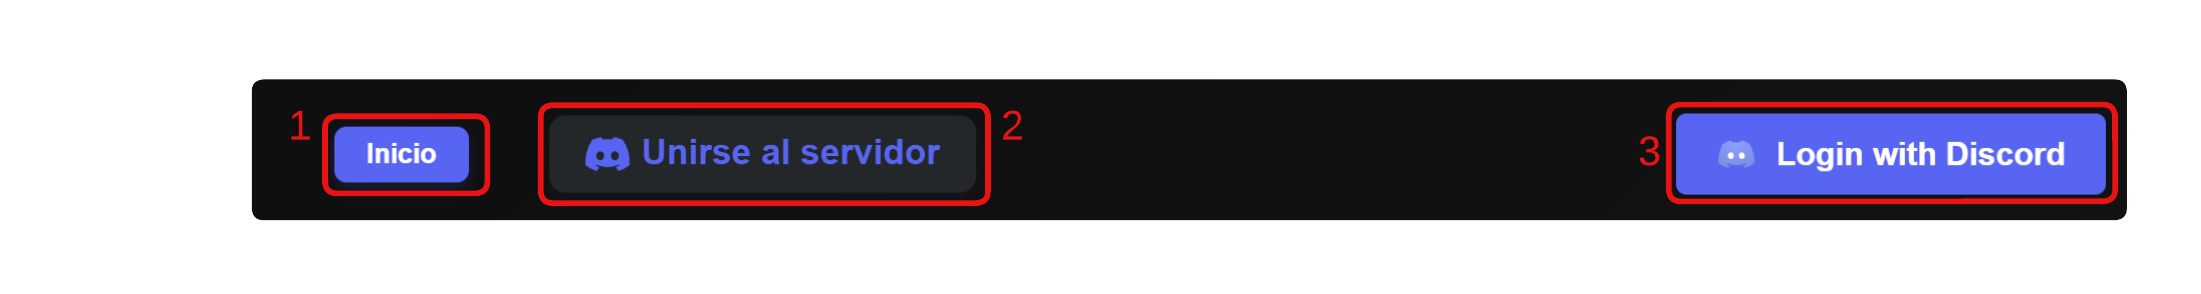
\includegraphics[width=1.0\textwidth]{./Imagenes/header1.png}
  \caption{Cabecera de la aplicación con botón de inicio de sesión}
  \label{fig:cabecera1}
\end{figure}

La figura~\ref{fig:cabecera1} muestra la cabecera de la aplicación, que incluye:\\
1. El botón de inicio, el cual llevará a la página principal de la tienda.\\
2. Un botón que desplegará una interfaz para acceder al servidor de Discord, la interfaz que abre se muestra en la Figura \ref{fig:servdiscord}.\\
3. Un botón que permitirá al usuario comenzar el registro o login mediante Discord, esta interfaz redirigirá al usuario a figura~\ref{fig:autorizacion}.

\subsubsection{Interfaz de Cabecera con Usuario Autenticado}
Esta interfaz mostrará la cabecera de la tienda virtual, esta cabecera se mostrará una vez el usuario inicie sesión.
\begin{figure}[H]
  \centering
  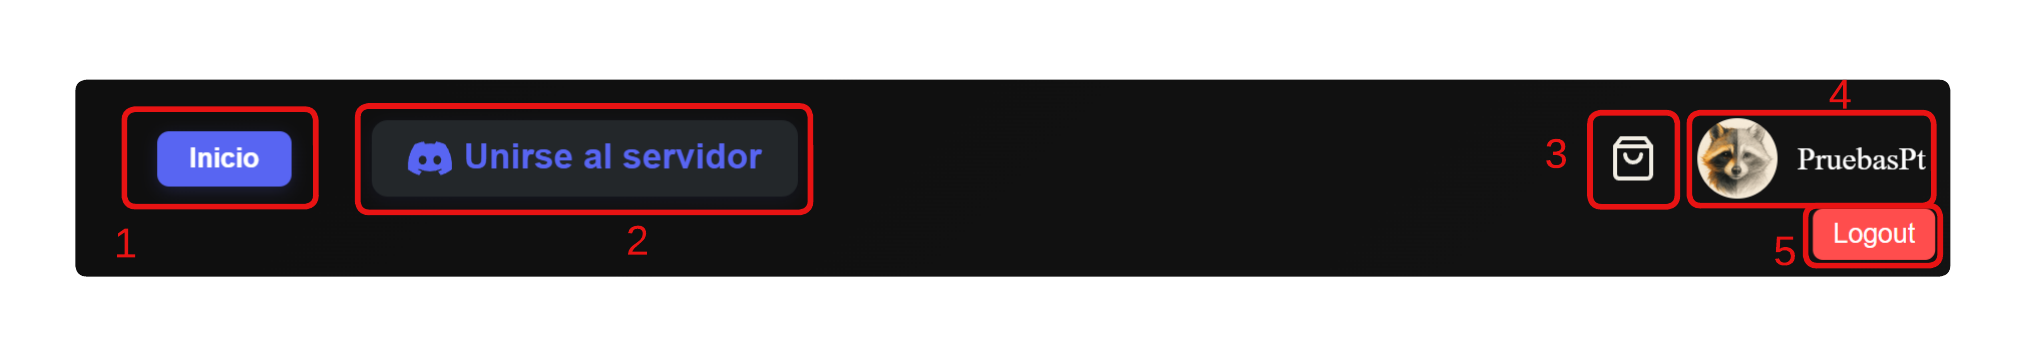
\includegraphics[width=1.0\textwidth]{./Imagenes/header2.png}
  \caption{Cabecera de la aplicación con usuario autenticado}
  \label{fig:cabecera2}
\end{figure}


La figura~\ref{fig:cabecera2} muestra la cabecera de la aplicación después del inicio de sesión de usuario. Los botones 1 y 2 de la cabecera no se modificarán, el botón 3 desaparecerá para ser reemplazado por:\\
3. El botón de carrito el cual le permitirá al usuario entrar a su interfaz de carrito.\\
4. Muestra el nombre del usuario y la imagen que tiene el usuario dentro de Discord.\\
5. Botón para cerrar sesión, el cual permitirá al usuario salir de su cuenta de Discord (se borra la cookie del usuario).

\subsubsection{Interfaz de Invitación a Discord}
La interfaz de invitación a Discord se mostrará al usuario una vez que dé clic en el botón 2 de la cabecera, este botón es el que permite al usuario unirse mediante código QR o el botón de invitación a Discord.
\begin{figure}[H]
  \centering
  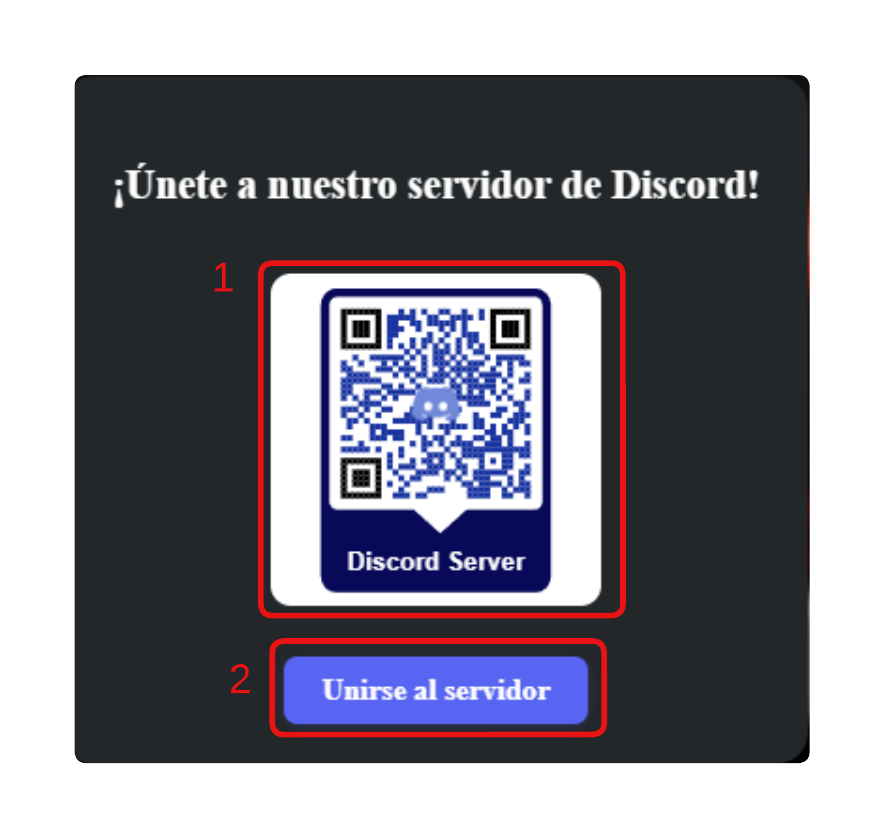
\includegraphics[width=0.8\textwidth]{./Imagenes/serverdiscord.png}
  \caption{Interfaz de invitación a Discord.}
  \label{fig:servdiscord}
\end{figure}
En la figura~\ref{fig:servdiscord} se pueden observar los siguientes elementos:\\
1. Un código QR que los usuarios pueden escanear para unirse al servidor de Discord.\\
2. Un botón que permite redirigir al usuario al servidor de Discord.\\

\subsubsection{Interfaz de Autenticación}
Esta interfaz muestra la ventana de autenticación de Discord que permite al usuario iniciar sesión en la aplicación.
\begin{figure}[H]
  \centering
  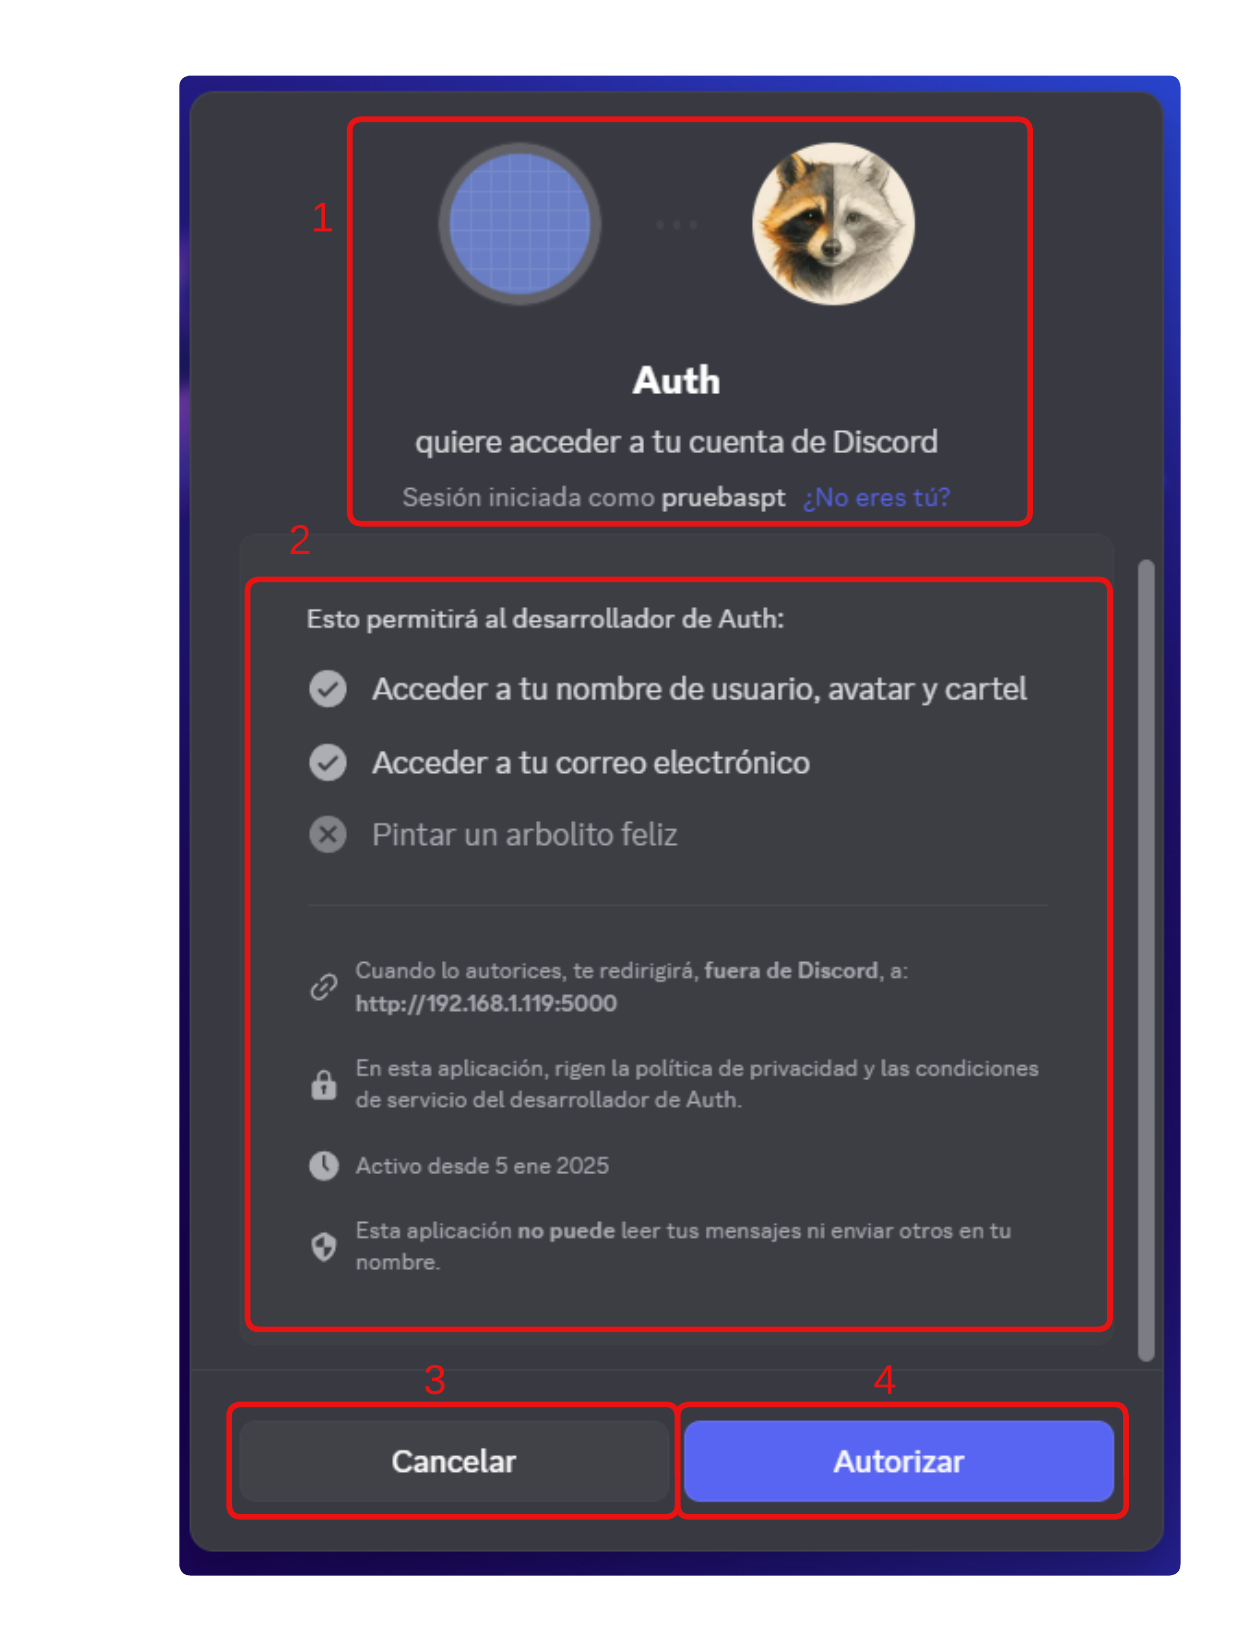
\includegraphics[width=0.8\textwidth]{./Imagenes/autorizacion.png}
  \caption{Vista de autorización de usuario}
  \label{fig:autorizacion}
\end{figure}
En la figura~\ref{fig:autorizacion} se pueden observar los siguientes elementos:\\
1. Se muestra la imagen que tiene el la imagen y el nombre de usuario de discord que hara el inicio de sesión.\\
2. Se enlistan los permisos que va a requerir la aplicacion.
3. Boton que le permite al usuario cancelar el inicio de sesión.
4. Boton de autorizar que le permite al usuario iniciar sesión en la aplicación.\\

\newpage
\subsubsection{Interfaz del Carrito con Productos}
Interfaz que se le mostrará al usuario cuando el carrito de compras tenga artículos seleccionados.
\begin{figure}[H]
  \centering
  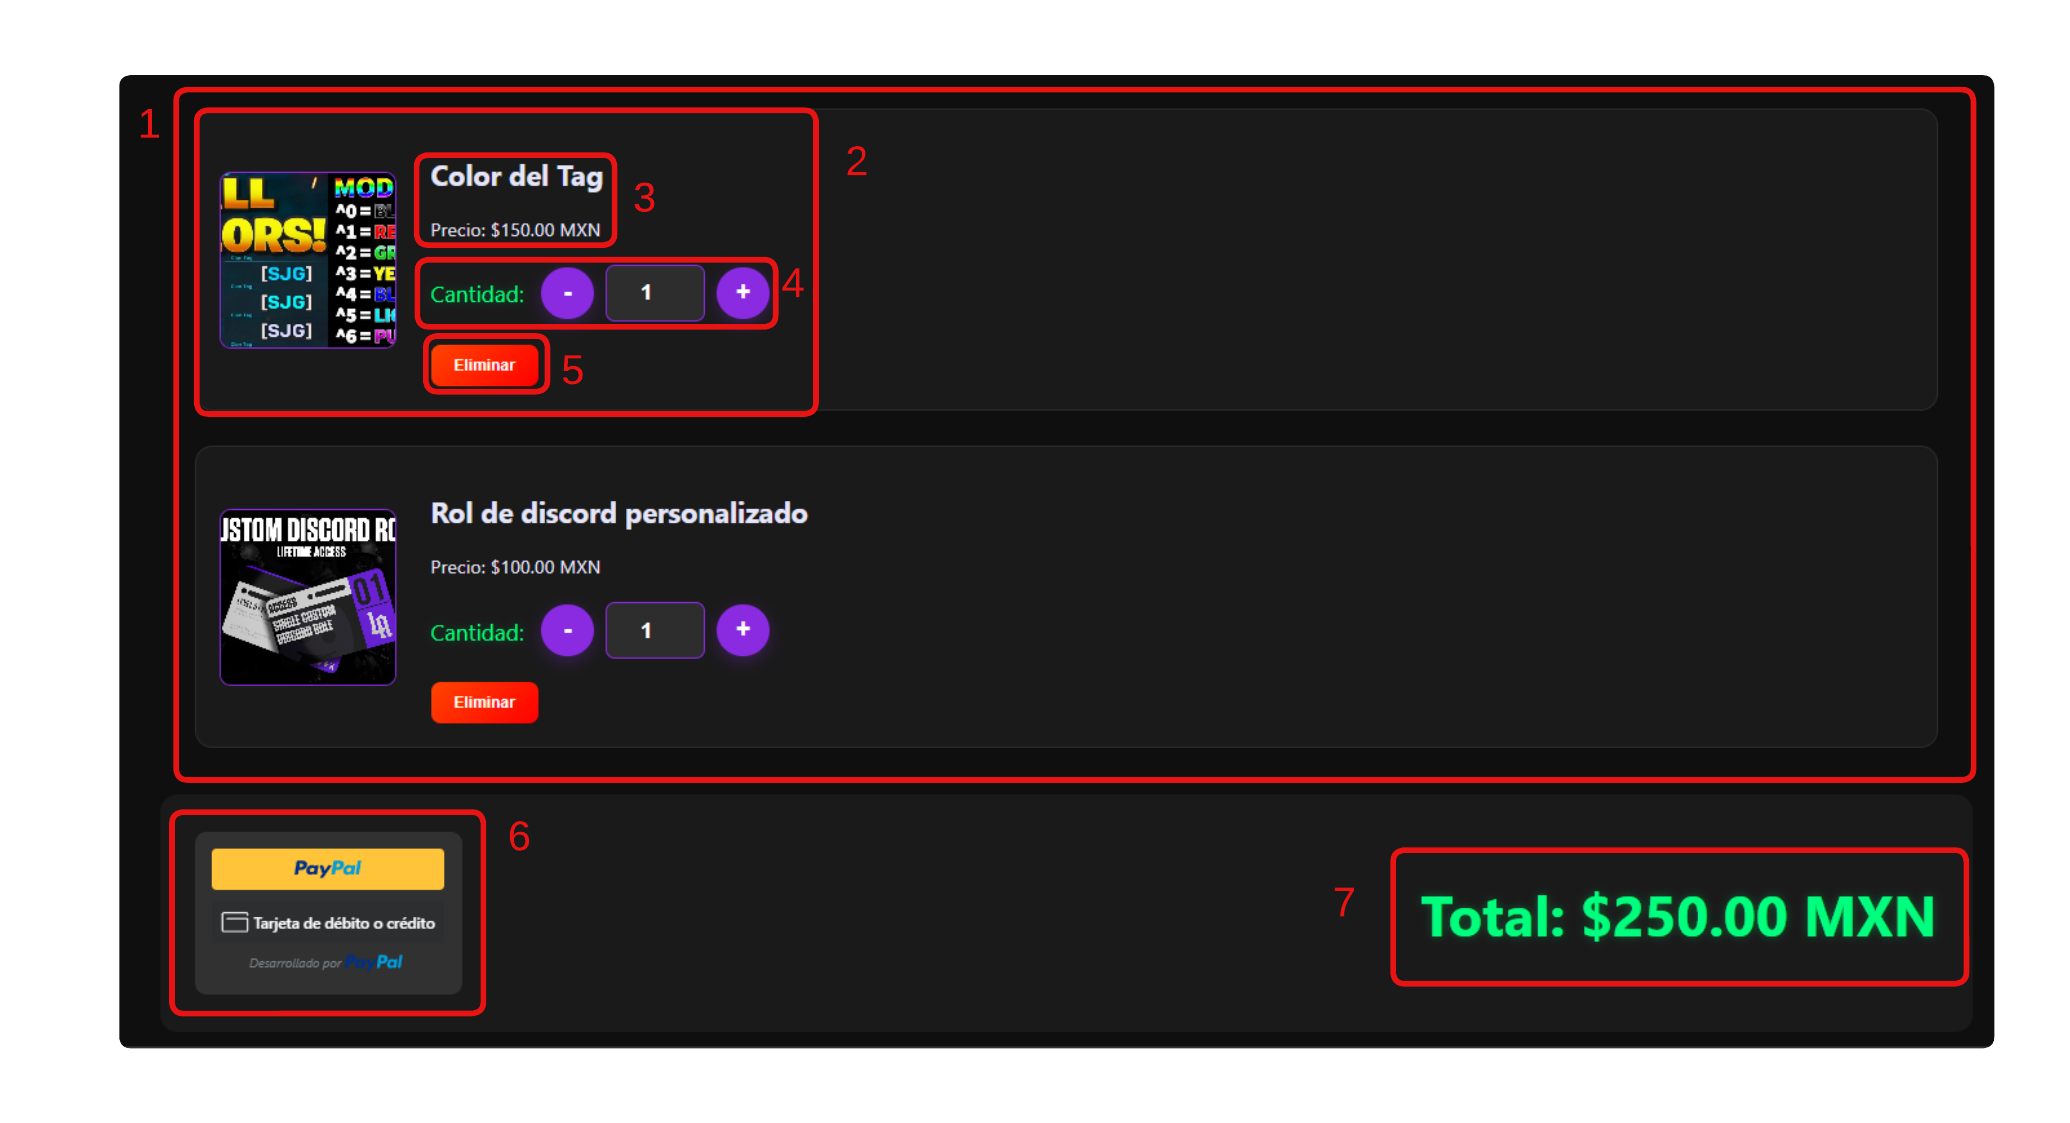
\includegraphics[width=0.8\textwidth]{./Imagenes/carrito_articulos.png}
  \caption{Vista del carrito de compras con productos}
  \label{fig:carritoprodu}
\end{figure}

En la figura~\ref{fig:carritoprodu} se pueden observar los siguientes elementos:\\
1. Lista de productos agregados al carrito.\\
2. Tarjeta del producto\\
3. Nombre y precio del producto\\
4. Control de cantidad de los productos dentro del carrito\\
5. Botón de eliminar el producto del carrito\\
6. Botón para iniciar la compra vía PayPal.\\
7. Precio total de la compra a realizar.\\

\subsubsection{Interfaz del Carrito Vacío}
Interfaz que se le mostrará al usuario cuando el carrito de compras esté vacio.
\begin{figure}[H]
  \centering
  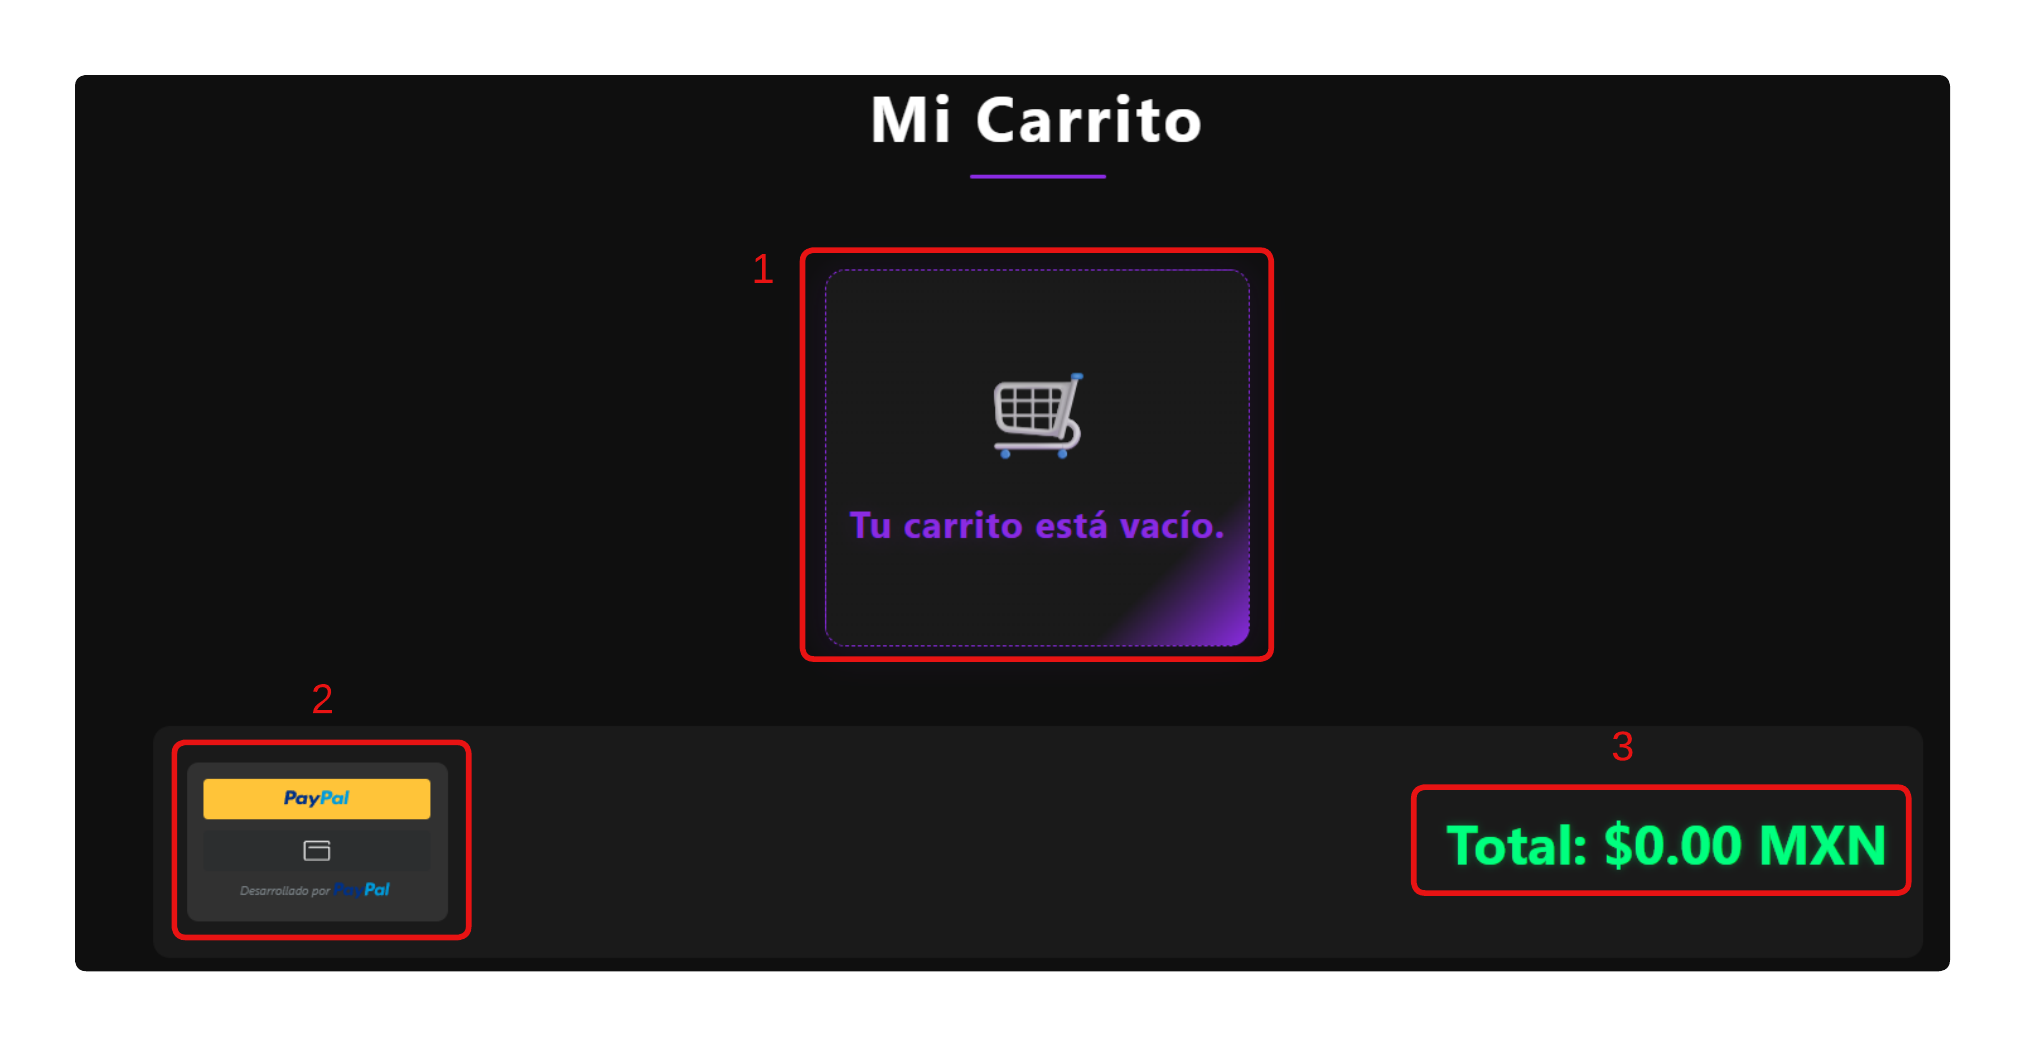
\includegraphics[width=0.8\textwidth]{./Imagenes/carrito_vacio.png}
  \caption{Vista del carrito de compras vacío}
  \label{fig:carritovacio}
\end{figure}

En la figura~\ref{fig:carritovacio} se pueden observar los siguientes elementos:\\
1. Botón con mensaje indicando que el carrito está vacío.\\
2. Botones de compra con PayPal, no dejará realizar compra si no hay artículos.\\
3. Total del valor de los artículos en el carrito\\

\subsubsection{Interfaz de busqueda de Productos}
En esta interfaz de mostrara la interfaz para que el usuario pueda comenzar a buscar productos y agregarlos al carrito
\begin{figure}[H]
  \centering
  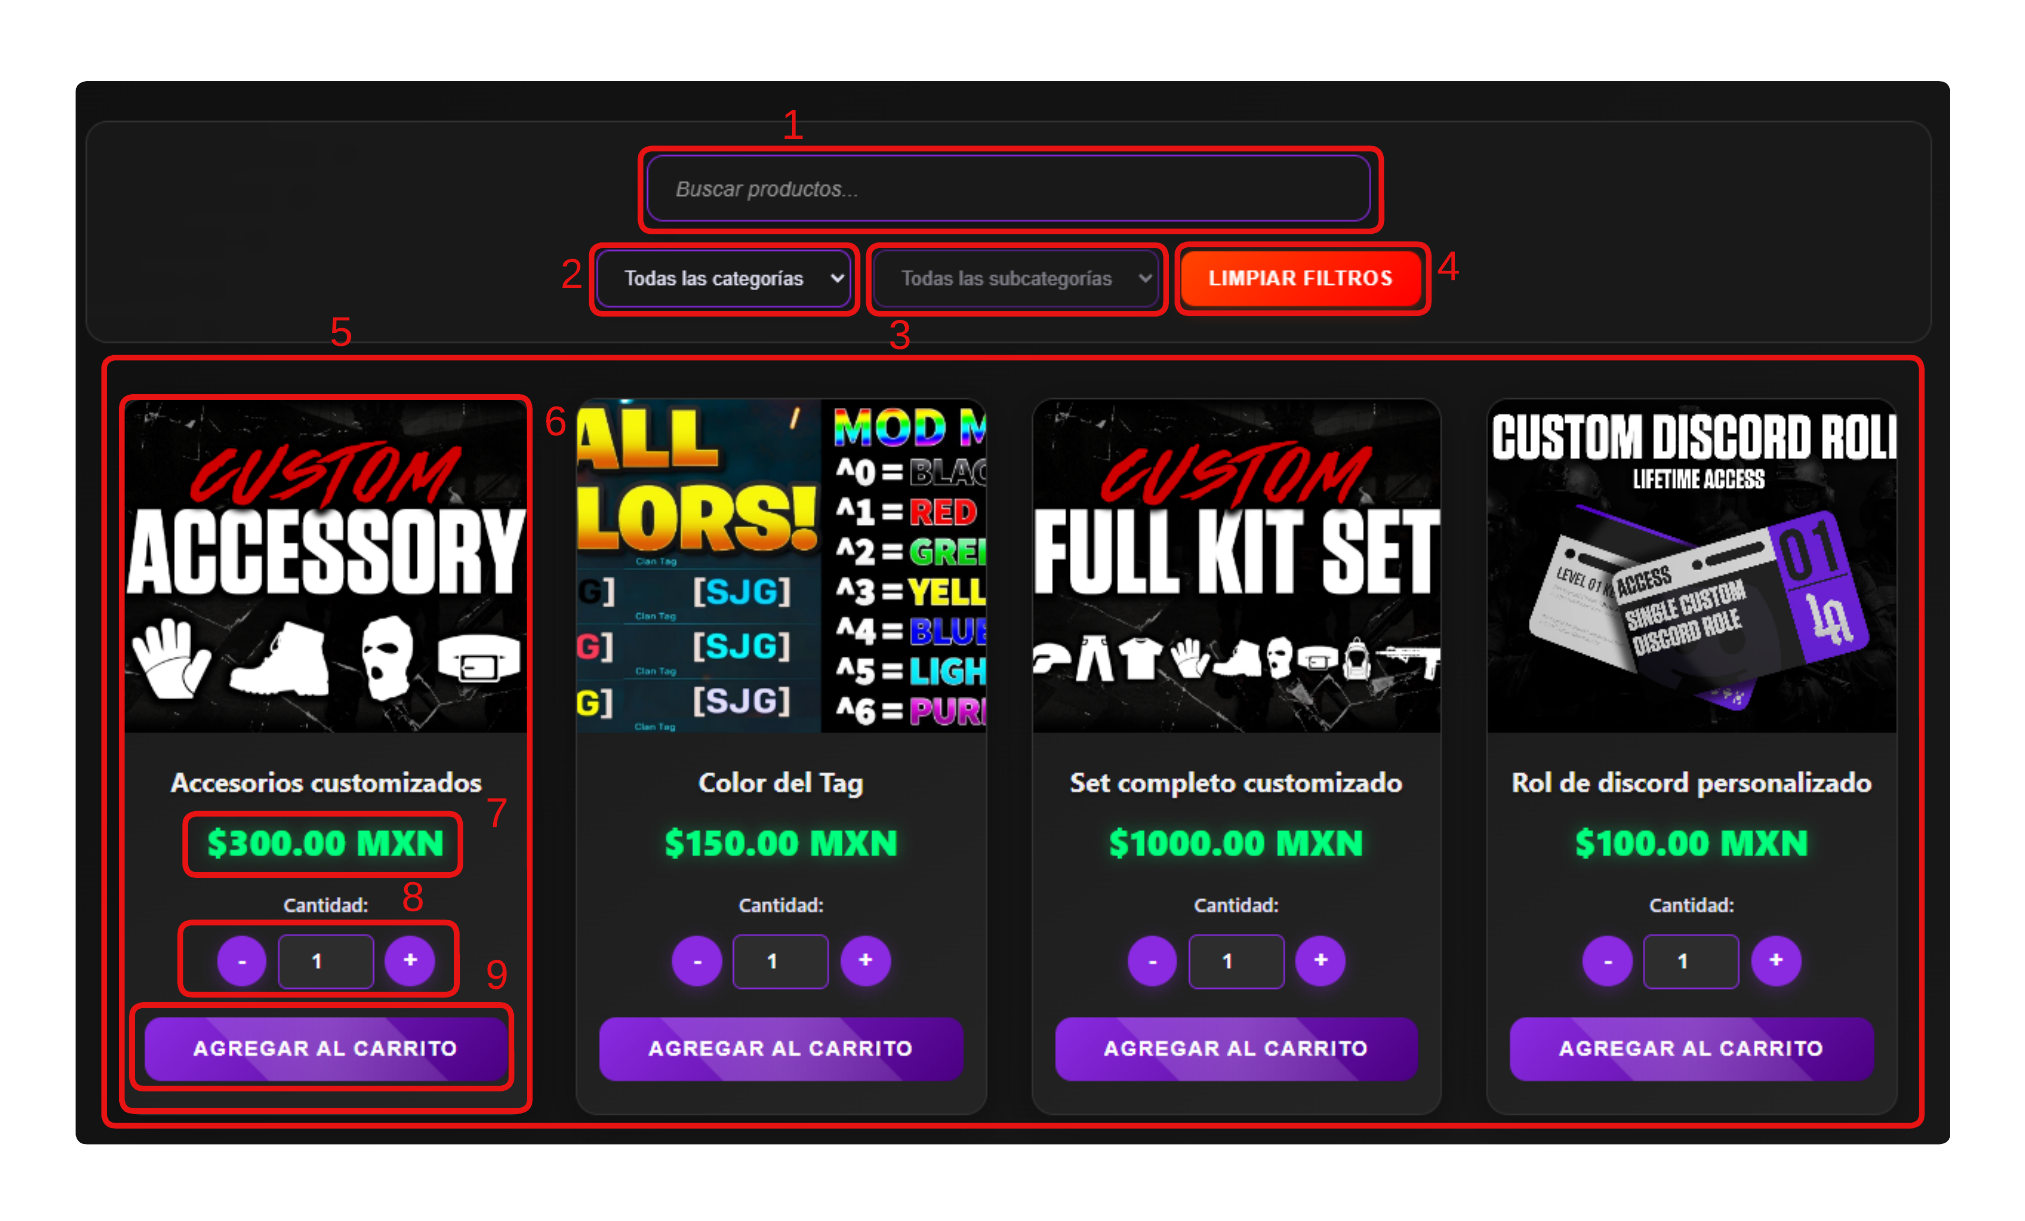
\includegraphics[width=0.8\textwidth]{./Imagenes/interproductos.png}
  \caption{Vista de la lista de productos y su filtro de búsqueda}
  \label{fig:interproductos}
\end{figure}

En la figura~\ref{fig:interproductos} se pueden observar los siguientes elementos:\\
1. Barra de búsqueda de productos por comparación de nombre ya sea parcial o total.\\
2. Menú desplegable de las categorías.\\
3. Menú desplegable de las subcategorías.\\
4. Botón para reiniciar los filtros de búsqueda.\\
5. Contenedor de los productos.\\
6. Tarjeta de cada producto con su información básica (imagen, nombre, precio, etc.).
7. Precio del producto.\\
8. Control de cantidad para el producto.\\
9. Botón para agregar el producto al carrito.\\



\subsection{Interfaces del Bot de Discord}
En esta seccion se mostraran las interfaces del bot asi como las interfaces de notificaciones via discord.
\newpage
\subsubsection{Creación de Comandos para Usuarios}
Instrucción que escribe el usuario en el chat de Discord.
\begin{figure}[H]
  \centering
  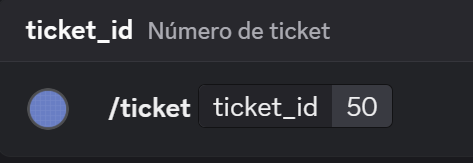
\includegraphics[width=0.6\textwidth]{./Imagenes/comandos.png}
  \caption{Comandos registrados del bot}
  \label{fig:comandos}
\end{figure}

La figura~\ref{fig:comandos} muestra el comando ticket que contiene el comando /ticket seguido de el \texttt{ticket\_id} y el número de ticket que el usuario quiera visualizar.

\subsubsection{Comprobación de Tickets Pendientes}
Es la interfaz del bot donde se podrá observar la comprobación constante que hace sobre los tickets pendientes así como la creación de canales para los tickets específicos.
\begin{figure}[H]
  \centering
  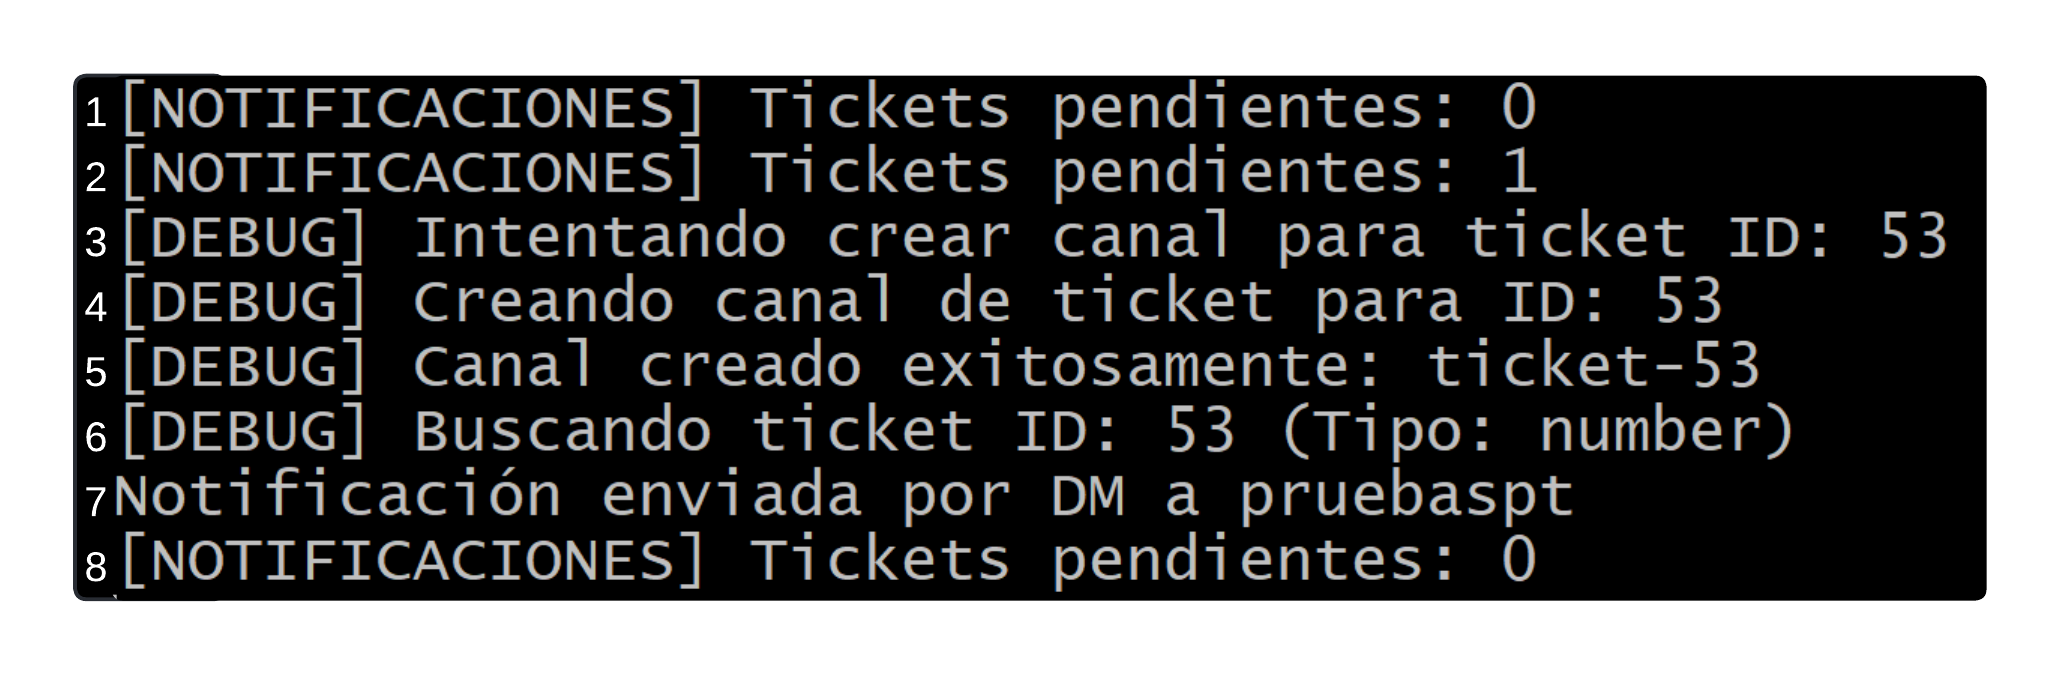
\includegraphics[width=0.8\textwidth]{./Imagenes/interbot.png}
  \caption{Verificación de tickets pendientes}
  \label{fig:tickets}
\end{figure}

En la figura~\ref{fig:tickets}, se pueden ver las siguientes acciones del bot:\\
Línea 1. Comprueba que no haya ningún ticket pendiente si el contador es 0 entonces no hay tickets por notificar.\\
Línea 2. Si el contador de tickets es 1 entonces comenzará el proceso de notificación automática.\\
Línea 3. Realiza las peticiones a la BD para comprobar los datos del ticket que no ha sido notificado.\\
Línea 4. Comienza la creación del canal para el ticket.\\
Línea 5. Crea exitosamente el canal privado con el usuario dueño del ticket.\\
Línea 6. Realiza la petición nuevamente para rescatar la información completa del ticket.\\
Línea 7. Envía un mensaje directo al usuario de que su canal para el ticket ha sido creado.\\
Línea 8. Una vez realizada la notificación el ticket cambia su estado a notificado y el bot continúa realizando la comprobación de tickets pendientes.\\

\subsubsection{Interfaz de Notificación vía Discord}
Interfaz de Discord donde el usuario podrá revisar su canal privado y la información de su ticket.
\begin{figure}[H]
  \centering
  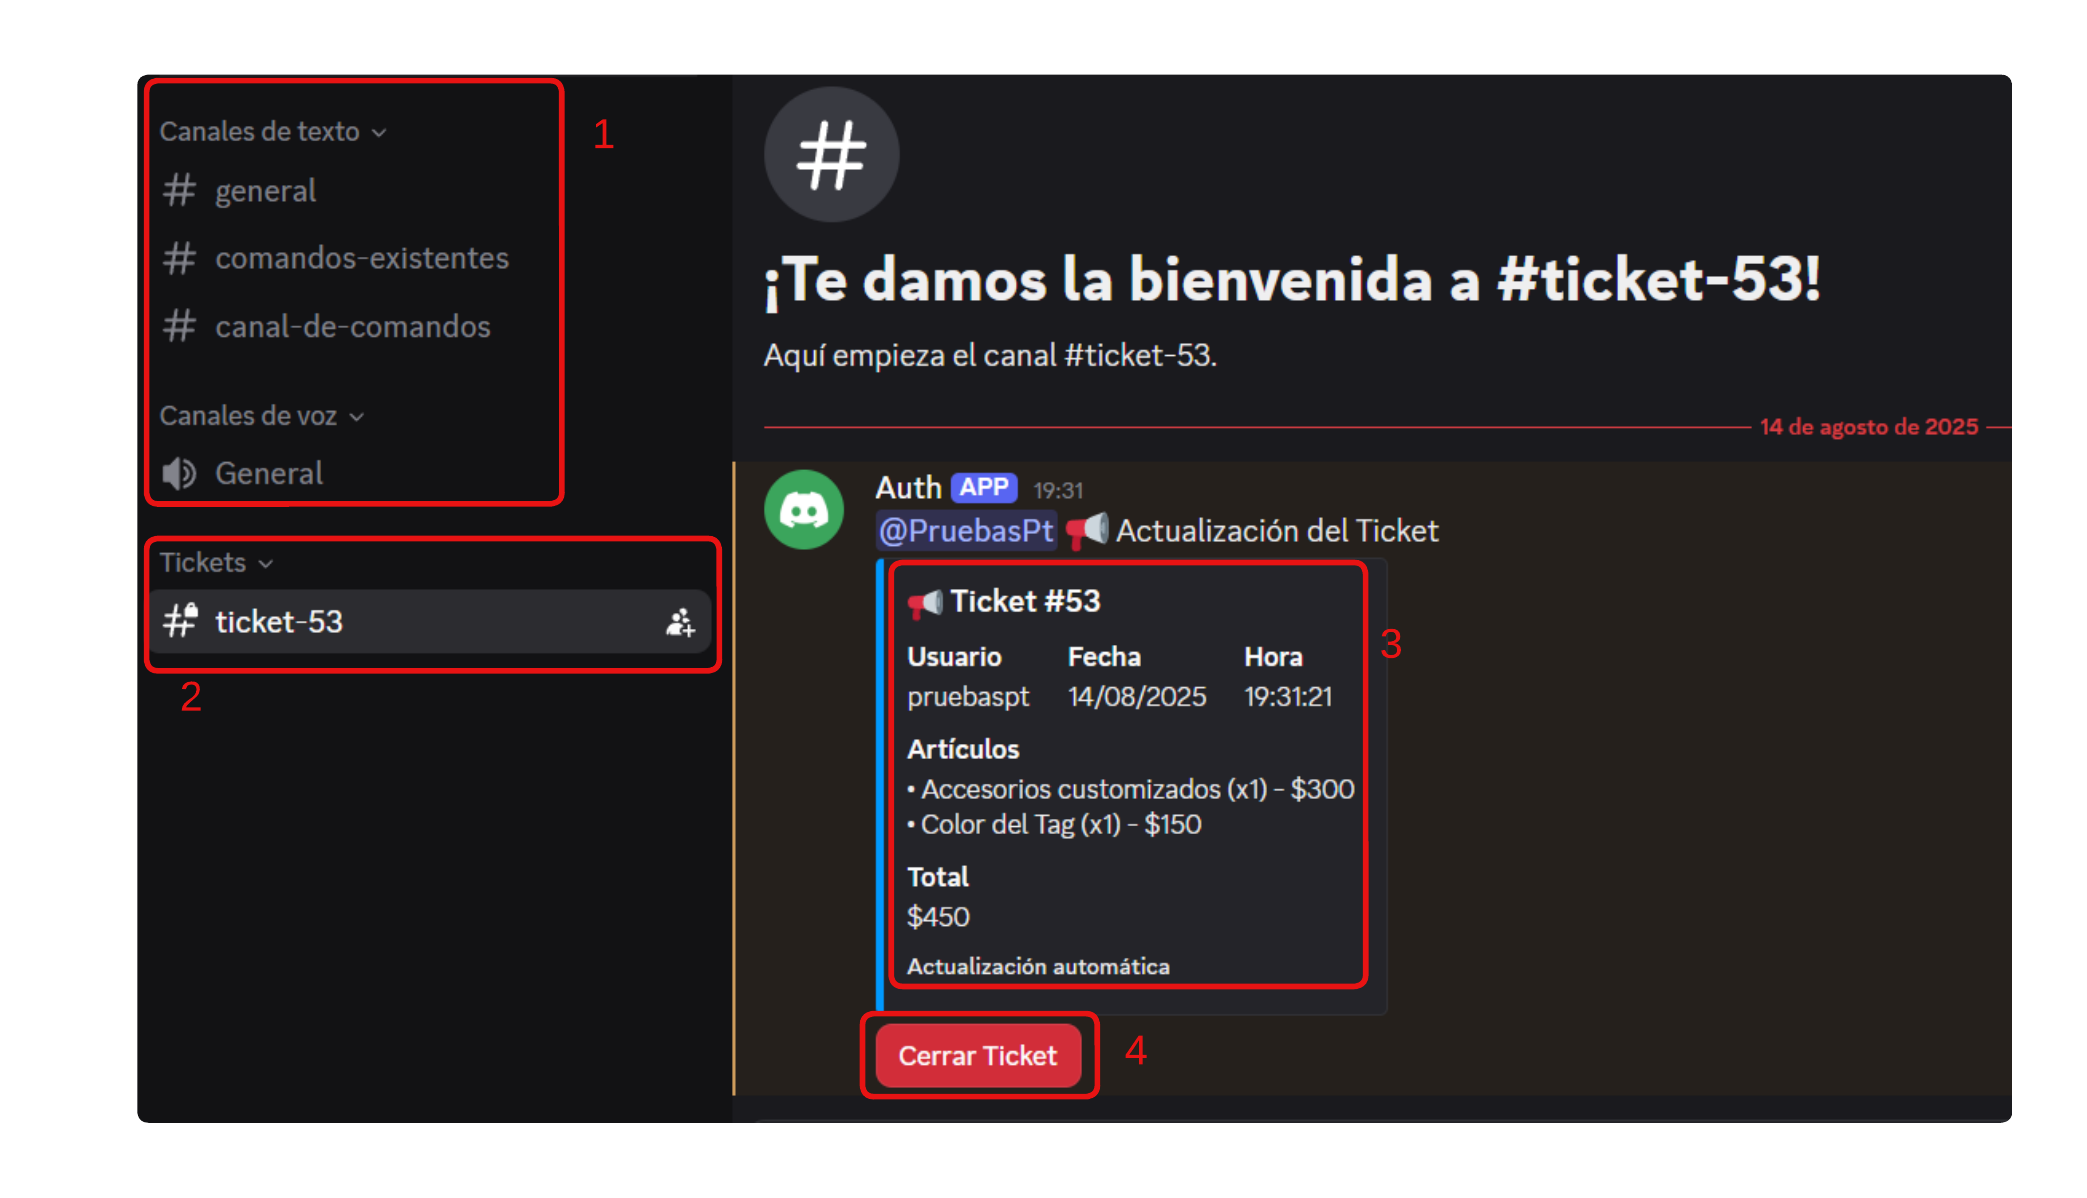
\includegraphics[width=1\textwidth]{./Imagenes/interdiscord.png}
  \caption{Notificación de ticket al usuario}
  \label{fig:tickets2}
\end{figure}

En la figura~\ref{fig:tickets2}, se muestra la interfaz de discord con las siguientes características:\\
1. Canales generales del servidor de Discord como los de mensajería y los de voz.\\
2. Categoría de tickets donde se crearán los canales para el ticket del usuario.\\
3. Información del ticket del usuario como nombre del comprador, fecha, hora, artículos comprados, precio, cantidad y total.\\
4. Boton que le permite al usuario o administrador cerrar el ticket.
\newpage
\subsubsection{Envío de Notificaciones por Canales Privados}
\begin{figure}[H]
  \centering
  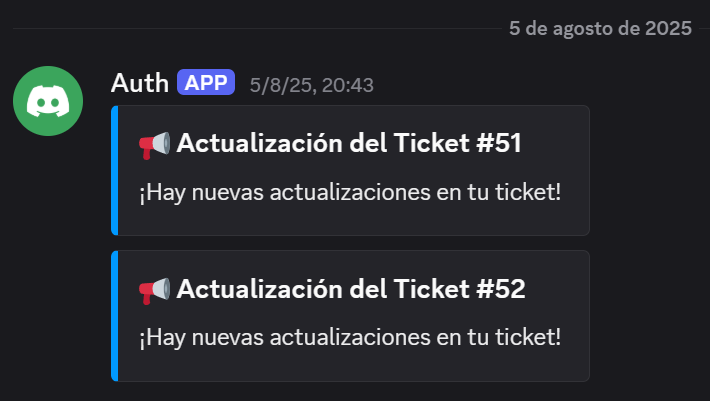
\includegraphics[width=0.6\textwidth]{./Imagenes/notificaciones.png}
  \caption{Mensaje privado de notificación}
  \label{fig:notificaciones}
\end{figure}

La figura~\ref{fig:notificaciones} ilustra cómo el bot envía notificaciones directas a los usuarios a través de mensajes privados en Discord. Estas notificaciones pueden incluir información sobre el estado de un pedido, recordatorios de pago o promociones especiales.

% --- Conclusiones ---
\newpage
\section{Conclusiones}

Durante el desarrollo de este proyecto se enfrentaron varios retos, especialmente el aprendizaje y uso de tecnologías nuevas como React para el frontend y la librería Discord.js para la integración del bot. Fue necesario revisar detalladamente la documentación para Discord.js que se encuentra en el Discord Developer Portal~\cite{discorddocs} y la documentación oficial de React~\cite{reactdocs}. Estos recursos fueron fundamentales para comprender cómo interactuar con la API de Discord y cómo construir una interfaz de usuario dinámica y responsiva.\\

Uno de los aspectos más importantes para este proyecto fue el diseño de la base de datos ya que tras varios rediseños en la base de datos se lograron integrar todas las funcionalidades requeridas para su correcto funcionamiento. También se requirió conseguir una serie de llaves API para poder interactuar con los servicios externos como Discord y PayPal.\\

Si bien se lograron incorporar todas las funcionalidades planteadas para este proyecto, sí faltaron algunas características que podrían mejorar la experiencia del usuario, como la creación de una interfaz para que el usuario pueda revisar todas las compras que ha realizado o un comando para Discord que le permita al usuario agregar productos al carrito desde Discord. Estas mejoras se consideran para futuras iteraciones del proyecto.\\

Un aspecto importante a considerar es la limitación impuesta por Discord en cuanto al envío de mensajes y notificaciones por parte de los bots. Discord establece límites estrictos en la cantidad de mensajes que un bot puede enviar en un período de tiempo determinado (rate limits). Por ejemplo, según la documentación oficial de Discord~\cite{discordlimits}, los bots pueden enviar hasta 5 mensajes por segundo por canal, y existen límites globales y por usuario que, si se superan, pueden llevar a que el bot sea temporalmente bloqueado o incluso baneado. Esto implica que, en escenarios donde se requiera notificar a un gran número de usuarios simultáneamente, el sistema debe implementar mecanismos de control y espera para evitar superar estos límites y garantizar la continuidad del servicio.


% --- Referencias ---
\newpage
\section{Referencias}
\begin{thebibliography}{12}
\bibitem{paypal} PayPal. Bienvenido a PayPal. Disponible en: \url{https://www.paypal.com/mx/webapps/mpp/welcome-to-paypal}. Accedido: 21-jun-2025.
\bibitem{mee6} MEE6. MEE6 - El bot de Discord más completo. Disponible en: \url{https://mee6.xyz/es}. Accedido: 21-jun-2025.
\bibitem{uniformes} R. Teja Rubio. Proyecto Tienda Virtual: Uniformes Escolares. UOC, 2016. Disponible en: \url{https://openaccess.uoc.edu/handle/10609/49345}
\bibitem{facebook} Facebook. Marketplace de Facebook. Disponible en: \url{https://www.facebook.com/marketplace/}. Accedido: 21-jun-2025.
\bibitem{aliexpress} AliExpress. Disponible en: \url{https://es.aliexpress.com/}. Accedido: 21-jun-2025.
\bibitem{campaignmonitor} Campaign Monitor. "Email Marketing Benchmarks and Statistics for 2023," Campaign Monitor, 2023. Disponible en: \url{https://www.campaignmonitor.com/resources/guides/email-marketing-benchmarks/}. Accedido: 21-nov-2024.
\bibitem{returnpath} Return Path. "2023 Deliverability Benchmark Report," Validity, 2023. Disponible en: \url{https://www.validity.com/resource-center/state-of-email-2023/}. Accedido: 21-nov-2024.
\bibitem{mma2023} Mobile Marketing Association. "Mobile Marketing Statistics and Trends 2023," MMA Global, 2023. Disponible en: \url{https://www.mmaglobal.com/research/mobile-marketing-statistics-2023}. Accedido: 21-nov-2024.
\bibitem{whatsappbusiness} WhatsApp Business. "WhatsApp Business API: Transforming Customer Communication," Meta for Business, 2023. Disponible en: \url{https://business.whatsapp.com/products/business-api}. Accedido: 21-nov-2024.
\bibitem{discorddocs} Discord Developer Portal. "Discord.js Documentation," Discord, 2024. Disponible en: \url{https://discord.js.org/#/docs/discord.js/stable/general/welcome}. Accedido: 15-dic-2024.
\bibitem{reactdocs} React Team. "React Documentation," Meta, 2024. Disponible en: \url{https://react.dev/learn}. Accedido: 15-dic-2024.
\bibitem{discordlimits} Discord Developer Portal. "Rate Limits," Discord, 2024. Disponible en: \url{https://discord.com/developers/docs/topics/rate-limits}. Accedido: 15-dic-2024.
\end{thebibliography}

\end{document}